\documentclass[12pt,oneside,english,a4paper]{article}
\usepackage{babel}
\usepackage[utf8]{inputenc}
\usepackage[T1]{fontenc}
\usepackage{color}
\usepackage{graphicx}
\usepackage{wallpaper}
\usepackage{wrapfig,booktabs}

\usepackage{fancyhdr}

\usepackage{fourier-orns}
\newcommand{\dash}{\noindent \newline\textcolor{black}{\hrulefill~ \raisebox{-2.5pt}[10pt][10pt]{\leafright \decofourleft \decothreeleft  \aldineright \decotwo \floweroneleft \decoone   \floweroneright \decotwo \aldineleft\decothreeright \decofourright \leafleft} ~  \hrulefill}}

\usepackage{titlesec}
\titleformat*{\section}{\it\huge\bfseries}
\titleformat*{\subsection}{\it\huge\bfseries}
\titleformat*{\subsubsection}{\it\LARGE\bfseries}
\titleformat*{\paragraph}{\huge\bfseries}
\titleformat*{\subparagraph}{\LARGE\bfseries}

\usepackage[left=20px,right=20px,top=50px,bottom=50px,paperwidth=8in,paperheight=12in]{geometry}


\usepackage[cjk]{kotex}

\usepackage{amsthm} 
\usepackage{amsmath} 
\usepackage{amsfonts}
\usepackage{enumerate} 
\usepackage{cite}
\usepackage{graphics} 
\usepackage{graphicx,lscape} 
\usepackage{subcaption}
\usepackage{algpseudocode}
\usepackage{algorithm}
\usepackage{titlesec}
\usepackage{cite, url}
\usepackage{amssymb}

\def\bk{\paragraph{\LARGE$$}\LARGE}
\def\ck{\paragraph{\LARGE$\bullet$}\LARGE}
\def\pf{\paragraph{\LARGE(pf)}\LARGE}
\def\note{\paragraph{\LARGE\textit{\underline{note:}}}\LARGE}
\def\ex{\paragraph{\LARGE\textit{example:}}\LARGE}
\newcommand{\para}[1]{\paragraph{\LARGE\it\underline{\textbf{#1:}}}\LARGE}
\newcommand{\parablue}[1]{\paragraph{\LARGE\textcolor{blue}{\it\underline{\textbf{#1:}}}}\LARGE}
\newcommand{\parared}[1]{\paragraph{\LARGE\textcolor{red}{\it\underline{\textbf{#1:}}}}\LARGE}
\newcommand{\paraviolet}[1]{\paragraph{\LARGE\textcolor{violet}{\it\underline{\textbf{#1:}}}}\LARGE}
\newcommand{\paraorange}[1]{\paragraph{\LARGE\textcolor{orange}{\it\underline{\textbf{#1:}}}}\LARGE}


\def\one{\paragraph{\LARGE(1)}\LARGE}
\def\two{\paragraph{\LARGE(2)}\LARGE}
\def\three{\paragraph{\LARGE(3)}\LARGE}
\def\four{\paragraph{\LARGE(4)}\LARGE}
\def\five{\paragraph{\LARGE(5)}\LARGE}
\def\six{\paragraph{\LARGE(6)}\LARGE}
\def\seven{\paragraph{\LARGE(7)}\LARGE}
\def\eight{\paragraph{\LARGE(8)}\LARGE}
\def\nine{\paragraph{\LARGE(9)}\LARGE}
\def\ten{\paragraph{\LARGE(10)}\LARGE}

\def\cka{\paragraph{\LARGE(a)}\LARGE}
\def\ckb{\paragraph{\LARGE(b)}\LARGE}
\def\ckc{\paragraph{\LARGE(c)}\LARGE}
\def\ckd{\paragraph{\LARGE(d)}\LARGE}
\def\cke{\paragraph{\LARGE(e)}\LARGE}
\def\ckf{\paragraph{\LARGE(f)}\LARGE}
\def\ckg{\paragraph{\LARGE(g)}\LARGE}
\def\ckh{\paragraph{\LARGE(h)}\LARGE}
\def\cki{\paragraph{\LARGE(i)}\LARGE}
\def\ckj{\paragraph{\LARGE(j)}\LARGE}

\newcommand{\bs}[1]{\mbox{\boldmath $#1$}}

\newcommand{\bsa}{\mbox{\boldmath $a$}}
\newcommand{\bsb}{\mbox{\boldmath $b$}}
\newcommand{\bsc}{\mbox{\boldmath $c$}}
\newcommand{\bsd}{\mbox{\boldmath $d$}}
\newcommand{\bse}{\mbox{\boldmath $e$}}
\newcommand{\bsf}{\mbox{\boldmath $f$}}
\newcommand{\bsg}{\mbox{\boldmath $g$}}
\newcommand{\bsh}{\mbox{\boldmath $h$}}
\newcommand{\bsi}{\mbox{\boldmath $i$}}
\newcommand{\bsj}{\mbox{\boldmath $j$}}
\newcommand{\bsk}{\mbox{\boldmath $k$}}
\newcommand{\bsl}{\mbox{\boldmath $l$}}
\newcommand{\bsm}{\mbox{\boldmath $m$}}
\newcommand{\bsn}{\mbox{\boldmath $n$}}
\newcommand{\bso}{\mbox{\boldmath $o$}}
\newcommand{\bsp}{\mbox{\boldmath $p$}}
\newcommand{\bsq}{\mbox{\boldmath $q$}}
\newcommand{\bsr}{\mbox{\boldmath $r$}}
\newcommand{\bss}{\mbox{\boldmath $s$}}
\newcommand{\bst}{\mbox{\boldmath $t$}}
\newcommand{\bsu}{\mbox{\boldmath $u$}}
\newcommand{\bsv}{\mbox{\boldmath $v$}}
\newcommand{\bsw}{\mbox{\boldmath $w$}}
\newcommand{\bsx}{\mbox{\boldmath $x$}}
\newcommand{\bsy}{\mbox{\boldmath $y$}}
\newcommand{\bsz}{\mbox{\boldmath $z$}}

\newcommand{\bfa}{\mbox{$\bf{a}$}}
\newcommand{\bfb}{\mbox{$\bf{b}$}}
\newcommand{\bfc}{\mbox{$\bf{c}$}}
\newcommand{\bfd}{\mbox{$\bf{d}$}}
\newcommand{\bfe}{\mbox{$\bf{e}$}}
\newcommand{\bff}{\mbox{$\bf{f}$}}
\newcommand{\bfg}{\mbox{$\bf{g}$}}
\newcommand{\bfh}{\mbox{$\bf{h}$}}
\newcommand{\bfi}{\mbox{$\bf{i}$}}
\newcommand{\bfj}{\mbox{$\bf{j}$}}
\newcommand{\bfk}{\mbox{$\bf{k}$}}
\newcommand{\bfl}{\mbox{$\bf{l}$}}
\newcommand{\bfm}{\mbox{$\bf{m}$}}
\newcommand{\bfn}{\mbox{$\bf{n}$}}
\newcommand{\bfo}{\mbox{$\bf{o}$}}
\newcommand{\bfp}{\mbox{$\bf{p}$}}
\newcommand{\bfq}{\mbox{$\bf{q}$}}
\newcommand{\bfr}{\mbox{$\bf{r}$}}
\newcommand{\bfs}{\mbox{$\bf{s}$}}
\newcommand{\bft}{\mbox{$\bf{t}$}}
\newcommand{\bfu}{\mbox{$\bf{u}$}}
\newcommand{\bfv}{\mbox{$\bf{v}$}}
\newcommand{\bfw}{\mbox{$\bf{w}$}}
\newcommand{\bfx}{\mbox{$\bf{x}$}}
\newcommand{\bfy}{\mbox{$\bf{y}$}}
\newcommand{\bfz}{\mbox{$\bf{z}$}}

\newcommand{\bsA}{\mbox{\boldmath $A$}}
\newcommand{\bsB}{\mbox{\boldmath $B$}}
\newcommand{\bsC}{\mbox{\boldmath $C$}}
\newcommand{\bsD}{\mbox{\boldmath $D$}}
\newcommand{\bsE}{\mbox{\boldmath $E$}}
\newcommand{\bsF}{\mbox{\boldmath $F$}}
\newcommand{\bsG}{\mbox{\boldmath $G$}}
\newcommand{\bsH}{\mbox{\boldmath $H$}}
\newcommand{\bsI}{\mbox{\boldmath $I$}}
\newcommand{\bsJ}{\mbox{\boldmath $J$}}
\newcommand{\bsK}{\mbox{\boldmath $K$}}
\newcommand{\bsL}{\mbox{\boldmath $L$}}
\newcommand{\bsM}{\mbox{\boldmath $M$}}
\newcommand{\bsN}{\mbox{\boldmath $N$}}
\newcommand{\bsO}{\mbox{\boldmath $O$}}
\newcommand{\bsP}{\mbox{\boldmath $P$}}
\newcommand{\bsQ}{\mbox{\boldmath $Q$}}
\newcommand{\bsR}{\mbox{\boldmath $R$}}
\newcommand{\bsS}{\mbox{\boldmath $S$}}
\newcommand{\bsT}{\mbox{\boldmath $T$}}
\newcommand{\bsU}{\mbox{\boldmath $U$}}
\newcommand{\bsV}{\mbox{\boldmath $V$}}
\newcommand{\bsW}{\mbox{\boldmath $W$}}
\newcommand{\bsX}{\mbox{\boldmath $X$}}
\newcommand{\bsY}{\mbox{\boldmath $Y$}}
\newcommand{\bsZ}{\mbox{\boldmath $Z$}}

\newcommand{\bfA}{\mbox{$\bf{A}$}}
\newcommand{\bfB}{\mbox{$\bf{B}$}}
\newcommand{\bfC}{\mbox{$\bf{C}$}}
\newcommand{\bfD}{\mbox{$\bf{D}$}}
\newcommand{\bfE}{\mbox{$\bf{E}$}}
\newcommand{\bfF}{\mbox{$\bf{F}$}}
\newcommand{\bfG}{\mbox{$\bf{G}$}}
\newcommand{\bfH}{\mbox{$\bf{H}$}}
\newcommand{\bfI}{\mbox{$\bf{I}$}}
\newcommand{\bfJ}{\mbox{$\bf{J}$}}
\newcommand{\bfK}{\mbox{$\bf{K}$}}
\newcommand{\bfL}{\mbox{$\bf{L}$}}
\newcommand{\bfM}{\mbox{$\bf{M}$}}
\newcommand{\bfN}{\mbox{$\bf{N}$}}
\newcommand{\bfO}{\mbox{$\bf{O}$}}
\newcommand{\bfP}{\mbox{$\bf{P}$}}
\newcommand{\bfQ}{\mbox{$\bf{Q}$}}
\newcommand{\bfR}{\mbox{$\bf{R}$}}
\newcommand{\bfS}{\mbox{$\bf{S}$}}
\newcommand{\bfT}{\mbox{$\bf{T}$}}
\newcommand{\bfU}{\mbox{$\bf{U}$}}
\newcommand{\bfV}{\mbox{$\bf{V}$}}
\newcommand{\bfW}{\mbox{$\bf{W}$}}
\newcommand{\bfX}{\mbox{$\bf{X}$}}
\newcommand{\bfY}{\mbox{$\bf{Y}$}}
\newcommand{\bfZ}{\mbox{$\bf{Z}$}}

\DeclareMathOperator*{\argmin}{argmin} 
\DeclareMathOperator*{\argmax}{argmax} 
\renewcommand{\footnotesize}{\fontsize{9pt}{11pt}\Large}

\usepackage[svgnames]{xcolor}
\usepackage{listings}

\lstset{language=R,
    basicstyle=\LARGE\tt,
    stringstyle=\color{DarkGreen},
    otherkeywords={0,1,2,3,4,5,6,7,8,9},
    morekeywords={TRUE,FALSE},
    deletekeywords={data,frame,length,as,character},
    %keywordstyle=\color{blue},
    commentstyle=\color{DarkGreen},
}
\CJKscale{0.9}
\begin{document}
\section{Markov Chain}

\paraorange{본문(챕터의목표)} The main object of study in this chapter is (temporally homogeneous) Markov chains on a countable state space $S$. That is, a sequence of r.v.'s $X_n, n\geq 0$, with 
\[
P(X_{n+1}=j | {\cal F}_n)=p(X_n,j)
\]
where ${\cal F}_n=\sigma(X_0,\dots,X_n), p(i,j)\geq 0$ and $\sum_jp(i,j)=1$. The theory focuses on the asymptotic behavior of 
\[
p^n(i,j)\overset{def}{=}P(X_n=j ~|~X_0=i).
\]
The basic results are that 
\[
\lim_{n\to\infty}\frac{1}{n}\sum_{m=1}^{n}p^m(i,j)\quad \mbox{exist always}
\]
and under a mild assumption called aperiodicity: 
\[
\lim_{n\to\infty}p^n(i,j)\quad \mbox{exists.}
\]
In nice situation, i.e., $X_n$ is irreduciable and positive recurrent, the limits in $\lim_{n\to\infty}\frac{1}{n}\sum_{m=1}^{n}p^{m}(i,j)$ and $\lim_{n\to\infty}p^{n}(i,j)$ are a probability distribution that is independent of the starting state $i$. In words, the chain converges to equilibrium\footnote{이퀼리브리움} as $n\to \infty$. One of the attractions of Markov chain theory is that these powerful conclusions come out of assumptions that are satisfied in a large number of cases. 


\paraviolet{해설} 이 챕터는 마코프체인의 수렴에 대하여 다룬다. 위에서 언급된 노테이션들이 이해가 잘 되지 않는다. 애초에 여기에서 $P$는 어떠한 확률공간에서 정의되는 메져인지도 불명확하다. 따라서 기호에 대한 해설들을 하겠다. 내가 나름대로 이해한 내용과 Random walks 앞부분을 참고하여 정리한바는 다음과 같다. 먼저 $\Omega$를 노드들의 집합이라고 하자. 즉 
\[
\Omega=\{{\tt node 1, node 2, \dots, node 24}\}
\]
그리고 걸음 $X_i$는 $(\Omega,{\cal F})$에서 정의되는 확률변수라고 하자. 즉 모든 $i\in\mathbb{N}$에 대하여 $X_i:(\Omega,{\cal F}) \to (S,{\cal S})$인 랜덤변수이다. 여기에서 $S=\{1,2,\dots,24\}$. \footnote{논의를 편하게 하기 위해서 $S=\mathbb{N}$ 혹은 $S=\mathbb{Z}$ 등을 사용할 수 있다. (어차피 카운터블만 다루므로 자연수나 정수로 맵핑한다.)} 이때 $X_1$과 $X_2$는 동일한 메저러블 스페이스 $(\Omega,{\cal F})$를 공유하지만 $X_1$, $X_2$가 같은 분포를 가질 필요는 없다. 그래서 $X_i$에 대응하는 확률공간은 $(\Omega,{\cal F},P_i)$이라고 볼 수 있다. 이때 의문인 점은 $X_i$ 각각에 대응하는 공간은 $(\Omega,{\cal F},P_i)$로 잘 정의되는데, 그럼 
\[
\bsX=[X_1,X_2,\dots]^\top
\]
와 같은 무한차원 확률벡터를 잘 정의시키는 확률공간도 존재할까? 라는 점이다.  일단 $X_1,X_2,\dots$이 \emph{iid}열이 아니므로 그렇게 쉽게 주장할 수 없어보인다. \textbf{하지만 일단 존재한다고 하자.} \footnote{원래 \emph{iid}열이면 콜모고로프 정리의 조건인 \textbf{"probability measures $\mu_n$ on $(\mathbb{R}^n,{\cal R}^{n})$ are consistent"}가 그냥 성립한다. 그래서 별 문제가 없이 무한차원으로 확장할 수 있다. 이 경우는 \emph{iid}열이 아니라서 그렇게 쉽지는 않아보인다. 그런데 $(S,{\cal S})$가 \textcolor{blue}{{\emph nice}}라면 무한차원으로 확장가능하다. 구체적인 내용은 다음 섹션 \textbf{Construction, Markov Properties}를 참고하라.} 그리고 이러한 확률공간을 $(\Omega_o,{\cal F}_{\infty},P)$라고 정의하자. 구체적으로는
\[
\Omega_o=\Omega \times \Omega \times \dots 
\]
\[
{\cal F}_{\infty}={\cal F}\times {\cal F} \times \dots 
\]
\[
P=P_1\times P_2\times \dots 
\]
가 된다. 즉 무한차원 확률변수열 $\bsX$에 대응하는 확률공간은 $(\Omega_o,{\cal F}_{\infty},P)$이다. 이제 앞으로 특별히 구분할 필요가 없다면 $\Omega=S$라고 하고 ${\cal F}={\cal S}$라고 하자. 따라서 앞으로는 $X_i:(S,{\cal S})\to(S,{\cal S})$인 확률변수이고 대응하는 확률공간은 $(S,{\cal S},P_i)$라고 보아도 무방하다. 따라서 이 논리대로라면 아래와 같이 볼 수 있다. 
\[
\Omega_o=S \times S \times \dots 
\]
\[
{\cal F}_{\infty}={\cal S}\times {\cal S} \times \dots 
\]
\[
P=P_1\times P_2\times \dots 
\]
 그리고 $\bsX:(\Omega_o,{\cal F}_{\infty}) \to (\Omega_o,{\cal F}_{\infty})$ 와 같이 볼 수 있다. 이제 무한열 $\bsX$에 대응하는 확률공간을 $(\Omega_o, {\cal F}_{\infty},P)$로 정의할 수 있다. {\bf 그리고 앞으로 특별한 언급이 없다면 이 공간을 항상 생각하자.} 마지막으로 몇 가지 노트들을 언급하겠다. 
\begin{enumerate}[(a)]
\item 본문에서 ${\cal F}_n$은 점점 커지는 시그마필드이다.
\item $P(X_{n+1}=j|{\cal F}_n)$은 $X_0,\dots,X_{n}$까지의 모든 정보가 given일 경우 즉 시점 $n$까지의 히스토를 모두 알고 있을 경우 $n+1$에 노드$j$를 방문할 (조건부)확률을 나타낸 것이다. \footnote{여기에서 $P$는 무려 무한열 $\bsX$에 대응하는 확률측도이다. 필요한 메져는 $P_{n+1 | 1,2,\dots,n}$ 즉 $X_{n+1}|{\cal F}_n$에 대응하는 확률측도인데 이는 $P$를 적당히 바꿔서 만들 수 있다.}
\item $p(X_n,j)=P(X_{n+1}=j|{\cal F}_n)$이다. 엄청 헷갈리는 기호이니까 나올때마다 바꿔주자. \footnote{여기에서 $p$역시 $P$에서 파생한것이므로 무한열 $\bsX$를 깔끔하게 정의할 수 있는 확률이다.}
\item $p(i,j)$는 아래와 같이 정의한다. (더렛의 Essentials of Stochastic Processes에서 참고) 
\[
p(i,j)\overset{def}{=}P(X_{n+1}=j ~|~ X_n=i,X_{n-1}=i_{n-1},\dots,X_0=i_0)
\]
\item 노드 $i$에서 출발한 아이가 어디든지 가긴 가야하므로 $\sum_{j}p(i,j)=1$이어야한다.  \footnote{좀더 구체적으로는 $\sum_{j\in S}p(i,j)=1$.} 즉 트랜지션매트릭스의 row-sum은 항상 1이다. \footnote{참고로 이러한 매트릭스를 스토캐스틱 매트릭스 혹은 마코프매트릭스라고 한다.}
\end{enumerate}

\para{의문} $\lim_{n\to\infty}p^n(i,j)$가 존재하면 항상 $\lim_{n\to\infty}\frac{1}{n}\sum_{m=1}^{n}p^m(i,j)$가 존재하지 않나? 왜냐하면 $0 \leq p^{n}(i,j)\leq 1$이니까?

\subsection{Definitions}
\paraorange{본문(마코프체인)} Let $(S,{\cal S})$ be a measurable space. A sequence of random variables taking values in $S$ is said to be a \textcolor{blue}{\bf Markov chain with respect to a filtration ${\cal F}_n$} if $X_n \in {\cal F}_n$ and for all $B \in {\cal S}$
\[
P(X_{n+1}\in B | {\cal F}_n)=P(X_{n+1}\in B |X_n)
\]
In words, given the present, the rest of the past is irrelevant for predicting the location of $X_{n+1}$. As usual, we turn to an example to illustrate the definition. 

\paraviolet{해설} 걸음열 $\{X_n\}$이 ${\cal F}_n$에 대한 마코프체인임을 보이기 위해서는 
\[
P(X_{n+1}\in B | {\cal F}_n)= P(X_{n+1}\in B |X_n)
\]
임을 보이면 된다고 한다. 쉽게말하면 $n+1$시점에 대한 확률분포(distribution)을 알기 위해서는 시점1부터 시점$n$까지 걸음열을 모두 기록한 정보 ${\cal F}_n=\sigma(X_0,X_1,X_2,\dots,X_n)$, 즉 $X_0,X_1,X_2\dots,X_n$에 해당하는 모든 자료가 필요한 것이 아니라 바로직전시점인 $n$시점의 자료 $X_n$만이 필요하다는 소리이다. 

\paraorange{Example 1.1 Random walk} Let $X_0,\xi_1,\xi_2,\dots \in \mathbb{R}^d$ be independent and let $X_n=X_0+\xi_1+\dots+\xi_n$. $X_n$ is a Markov chain with respect to ${\cal F}_n=\sigma(X_0,X_1,\dots,X_n)$. (As in the case of a martingale, this is the smallest filtration we can get away and the one we will usually use.) To prove our claim, we want to show that if $\mu_j$ is the distribution of $\xi_j$, then 
\[
P(X_{n+1} \in B | {\cal F}_n)=\mu_{n+1}(B-X_n)=P(X_{n+1}\in B|X_n)
\]
To prove the first equality, we note that $X_n$ and $\xi_{n+1}$ are independent and use following example. 
\para{(Example in Chap. Martingales)} Suppose $X$ and $Y$ are independent. Let $\varphi$ be a function with $E|\varphi(X,Y)|<\infty$ and let $g(x)=E(\varphi(x,Y))$. Then 
\[
E(\varphi(X,Y)|X)=g(X)
\]
The second equality follows from: 
\para{Lemma} If ${\cal F}\subset {\cal G}$ and $E(X|{\cal G})\in {\cal F}$ then $E(X|{\cal F})=E(X|{\cal G})$.

\paraviolet{해설} 오차합(=랜덤워크)는 항상 마코프체인이다. 

\subsection{Construction}
\paraorange{본문} Our next goal is to take the rather abstract object defined at the beginning of the section and, without loss of generality, turn it into something more concrete and easier to work with. We begin with two definitions: A function $p: S\times {\cal S} \to \mathbb{R} $ is said to be a \textcolor{blue}{\bf transition probability} if 
\begin{enumerate}[(i)]
	\item For each $x \in S, A\to p(x,A)$ is a probability measure on $(S,{\cal S}).$
	\item For each $A \in {\cal S}$, $x\to p(x,A)$ is measurable function. 
\end{enumerate}
We say $X_n$ is a Markov chain (w.r.t. ${\cal F}_n$) with transition probabilities $p_n$ is 
\[
P(X_{n+1}\in B|{\cal F}_n)=p_n(X_n,B)
\]

\paraviolet{해설} 어떠한 함수 $p:S\times {\cal S} \to \mathbb{R}$이 transition probability라고 불리기 위해서 어떠한 조건들이 필요한지 설명한다. 본문의 내용을 이해하는 것이 좀 어려운데 그 이유는 $p(x,A)$의 기호가 너무 어렵기 때문이다. 따라서 여기에서 $p(x,A)$의 의미를 잘 파악하는 훈련을 해볼것이다. $p(x,A)$의 뜻은 노드 $x$에서 출발하여 그 다음에 $A$중 하나의 원소로 이동할 확률을 의미한다. \footnote{$A\subset S$는 노드들의 집합임.} 이 기호를 좀 더 이해하기 위해 익숙한 $4\times 4$ 그리드 세계를 가정하자. $\Omega={\tt \{node 1,node 2,\dots,node 16\}}$이고 $S=\{1,2,\dots,16\}$이라고 하자. 확률변수 $X_1:(\Omega,{\cal F}) \to (S, {\cal S})$은 아래와 같이 정의할 수 있는 맵핑이라고 하자.\footnote{혹은 $X_1:(\Omega,{\cal F}) \to (\mathbb{R},{\cal R})$}
\begin{align*}
X_1\big({\tt node 1}\big)=1, \quad \dots \quad X_1\big({\tt node 16}\big)=16
\end{align*}
이제 ${\tt node1}$\footnote{ 즉 ${\tt location~ (1,1)}$} 의 위치에서 ${\tt node2}$의 위치로 이동하는 transition probability를 $p:S\times {\cal S} \to \mathbb{R}$라고 정의하자.\footnote{출발은 $S$ 도착은 ${\cal S}$인 셈이다.}  $S$의 원소는 노드이지만 ${\cal S}$의 원소는 노드들의 집합이다. 따라서 $p$는 아래와 같이 쓰는 것이 바람직하다. 
\[
p(x,A), \quad x \in S \mbox{ and } A \in {\cal S}
\]
$x$와 $A$를 잘 구분하는 것이 매우 중요하다. 아래를 관찰하여 그 차이를 명확하게 하자. 
\begin{enumerate}[(a)]
\item $x=1  \Longleftrightarrow  X(\omega)=1  \Longleftrightarrow  \omega={\tt node1}$
\item $A=\{1,2,5\}  \Longleftrightarrow  \{\omega:X(\omega) \in A\}=\{{\tt node1,node2,node5}\}$
\end{enumerate}
따라서 $p(1,\{1,2,5\})$의 의미는 ${\tt node1}$에서 출발한 걸음이 바로 다음턴에 ${\tt \{node1, node2, node5\}}$중 하나에 도착할 확률을 의미한다. 

\paraorange{본문(nice, Kolmogorov's theorem)} When $(S,{\cal S})$ is nice, supposing the existence of a transition probability entails no loos of generality, since the Markov property asserts that the conditional expectation w.r.t. ${\cal F}_n$ is same as w.r.t. $\sigma(X_n)$, and then following exercise implies the existence of a transition probability.
\para{(Exercise in Chap. Martingale)} Suppose $X$ and $Y$ take values in a nice space $(S,{\cal S})$ and ${\cal G}=\sigma(Y)$. Then there is a function $\mu:S \times {\cal S} \to [0,1]$ so that 
\begin{enumerate}[(i)]
	\item for each $A$, $\mu(Y(\omega),A)$ is a version of $P(X\in A | {\cal G})$. 
	\item for a.e. $\omega$, $A \to \mu(Y(\omega),A)$ is a probability measure on $(S,{\cal S})$.
\end{enumerate}
Conversely, if we suppose $(S,{\cal S})$ is a nice space, then given a sequence of transition probabilities $p_n$ and an \textcolor{blue}{\bf initial distribution $\mu$} on $(S,{\cal S})$, we can define a \textcolor{blue}{consistent set of finite dimensional distribution} by 
\begin{align*}
& \textcolor{blue}{P(X_j\in B_j, 0\leq j\leq n)}\\ 
& =\int_{B_0}\mu(dx_0)\int_{B_1}p_0(x_0,dx_1)\dots\int_{B_n}p_{n-1}(x_{n-1},dx_n)
\end{align*}

\paraviolet{해설} 정리하면 다음과 같은 스토리 흐름이다. (1) $(S,{\cal S})$이 nice space 이다. (2) 그러면 모든 $n$에 대하여 $p_n$이 잘 정의된다. (Exercise in Chap. Martingale) (3) 그럼 이제 잘정의되는 초기분포 $\mu$와 $p_n$을 가지고 있는데 이것으로 consistent set of finite dimensional distribution 을 잘 정의할 수 있다. \footnote{원래는 (1) $\mu$와 $p_n$으로 정의되는 $X_n$이 마코프체인임을 보인뒤에 (정리 5.2.1, 5판) (2) $X_n$이 마코프체인 (with $\mu$ and $p_n$) 일때 consistent한 finite dimensional distribution을 가짐(정리 1.3, 3판)을 보이는 것이 정식 스토리이다. 여기는 조금 생략된 버전임.}

\paraorange{본문} Since we have assumed that $(S,{\cal S})$ is nice, Kolmogorov's theorem allows us to construct a probability measure \textcolor{blue}{$P_{\mu}$} on sequence space 
\[
(\Omega_o,{\cal F}_{\infty})=\Big(S^{\{0,1,\dots\}},{\cal S}^{\{0,1,\dots\}}\Big)
\] 
so that the coordinate maps $X_n(\omega)=\omega_n$ have the desired distributions. 

\para{Notation} When $\mu=\delta_x$, a point mass at $x$, we use $P_x$ as an abbreviation for $P_{\delta_x}$. The measures $P_x$ are the basic objects because, once they are defined, we can define the $P_{\mu}$ (even for infinite measure $\mu$) by 
\[
P_{\mu}(A)=\int \mu(dx)P_x(A)
\]

\paraviolet{해설} $P_{x}(A)$는 초기분포가 $\mu=\delta_x$일 경우 \footnote{즉 랜덤워크의 첫 시작이 노드 $x$일 경우} 어떠한 event $A$가 일어날 확률을 의미한다. 여기에서 $P_{\mu}$ or $P_{x}$는 $(\Omega_o,{\cal F}_{\infty})$에서의 메져이므로 이벤트 $A$의 예는 아래와 같다. 
\begin{align*}
& X_1 =1 ,X_2 \in \{2,3\},X_3 \in \mbox{set of all node}, X_4=1 \dots \\
& \Leftrightarrow A=\{{\tt node1} \}\times \{{\tt node2,node3}\} \times S \times \{{\tt node1} \} \times \cdots
\end{align*}
즉 무한열 $\bsX$에 대한 모든 걸음들을 정의할 수 있는 사건을 의미한다. 따라서 $P_{x}(A)$ 는 예를들어 아래와 사건에 대한 확률을 정의할 수 있는 메져이다. 
\begin{align*}
n=0: & \quad \mbox{\textbf{처음에 노드$x$에서 시작}} \\
n=1: & \quad \mbox{노드1로 이동} \\
n=2: & \quad \mbox{노드2,3 중 하나로 이동} \\
n=3: & \quad \mbox{아무곳이나 이동} \\
n=4: & \quad \mbox{노드1로 이동} \\
\dots 
\end{align*}
따라서 $\int_x \mu(dx)P_x(A)$는 $n=0$시점에서 초기분포가 노드 $x$에서 시작되는것이 아닌 어떠한 임의의 분포 $\mu$를 가질 경우 \footnote{예를들면 노드 1에 있을 확률이 $1/2$이고 노드 2에 있을 확률이 $1/2$이라는 식의 분포} 위와 같은 확률을 잘 정의할 수 있는 장치이다. 즉 $P_{\mu}(A)$는 랜덤워크의 처음위치가 $\mu$와 같은 분포를 따를때 사건 $A\in {\cal F}_{\infty}$가 일어날 확률을 의미한다. 

\paraorange{Theorem 5.2.1 (5판)} Our next step is to check that $X_n$ is a Markov chain with respect to ${\cal F}_n=\sigma(X_0,X_1,\dots,X_n)$ with transition probability $p_n$. That is, 
\[
P_{\mu}(X_{n+1}\in B | {\cal F}_n) = p_n(X_n,B)
\]

\paraviolet{해설} 즉 transition probability $p_n$으로 정의되는 걸음열 $\bsX=\{X_n\}$는 마코프체인이라는 것이다. 

\paraorange{Theorem 1.3 (3판)} if $X_n$ is a Markov chain with transition probabilities $p_n$ and initial distribution $\mu$, then the finite dimensional distribution are given by
\begin{align*}
&P(X_j\in B_j, 0\leq j\leq n) \\
&=\int_{B_0}\mu(dx_0)\int_{B_1}p_0(x_0,dx_1)\dots\int_{B_n}p_{n-1}(x_{n-1},dx_n)
\end{align*}
\dash 
\para{정리 1.3의 증명}
\para{공식} Our next small step is to show that if $X_n$ has transition probability $p_n$ then for any bounded measurable $f$
\[
E(f(X_{n+1})|{\cal F}_n) = p_n(X_n, dy)f(y) \quad \cdots (\star) \footnote{$f(X_{n+1})$은 노드에 값이 매겨진 것이니까 그래프 신호라고 보아도 무방하다. 그러니까 $f:S \to \mathbb{R}$}
\]
The desired conclusion is a consequence of the next result which will save
us work in later proofs. Let ${\cal H} =$ the collection of bounded functions for which the identity holds. 

\para{Monotone class theorem} Let ${\cal A}$ be a $\pi$-system that
contains $\Omega$ and let ${\cal H}$ be a collection of real-valued functions that satisfies: 
\begin{enumerate}[(i)]
\item If $A \in{\cal A}$, then $1_A \in {\cal H}$.
\item If $f,g \in {\cal H}$, then $f + g$, and $cf \in {\cal H}$ for any real number $c$.
\item If $f_n \in {\cal H}$ are nonnegative and increase to a bounded function $f$, then $f \in {\cal H}$.
\end{enumerate}
Then ${\cal H}$ contains all bounded functions measurable with respect to $\sigma({\cal A})$.

\ck Returning to our main topic, we observe that familiar properties of 
conditional expectation and $(\star)$ imply 
\begin{align*}
&E\left(\prod_{m=0}^{n}f_m(X_m)\right)=E~ \textcolor{red}{E} \left(\prod_{m=0}^{n}f_m(X_m)\bigg | {\cal F}_{n-1}\right) \\ 
&= E \left(\prod_{m=0}^{n-1}f_m(X_m)\textcolor{red}{E}\left(f_n(X_n) \big| {\cal F}_{n-1}\right)\right) \\
&= E \left(\prod_{m=0}^{n-1}f_m(X_m)\int p_{n-1}(X_{n-1},dy)f_n(y)\right)  
\end{align*}
The last integral is a bounded measurable function of $X_{n-1}$, so it follows by induction that if $\mu$ is the distribution of $X_0$, then
\begin{align*}
E\left(\prod_{m=0}^{n}f_m(X_m)\right)=& \int\mu(dx_0)f_0(x_0)\int p_0(x_0,dx_1)f_1(x_1)\\ 
& \cdots\int p_{n-1}(x_{n-1},dx_n)f_n(x_n)
\end{align*}
that is, the finite dimensional distributions coincide with 
\begin{align*}
&P(X_j\in B_j, 0\leq j\leq n)\\
&=\int_{B_0}\mu(dx_0)\int_{B_1}p_0(x_0,dx_1)\dots\int_{B_n}p_{n-1}(x_{n-1},dx_n)
\end{align*}

\paraviolet{해설} 정리 1.3은 $X_n$이 잘 정의된 $p_n$과 $\mu$를 가진 마코프체인이라면 항상 일관성있는 (consistent한, 즉 콜모고로프정리를 쓰기에 적합한) finite dimensional distribution을 정의할 수 있다는 의미이다. 

\paraorange{본문} With Theorem 1.3 established, it follows that we can describe a Markov chain by giving a sequence of transition probabilities $p_n$. Having done this, we can and will suppose that the random variables $X_n$ are the coordinate maps $(X_n(\omega) =\omega_n)$ on sequence space
\[
(\Omega_o,{\cal F}_{\infty})=\Big(S^{\{0,1,\dots\}},{\cal S}^{\{0,1,\dots\}}\Big)
\]
We choose this representation because it gives us two advantages in investigating the Markov chain: (i) For each initial distribution $\mu$ we have a measure $P_{\mu}$ defined by 
\begin{align*}
&P(X_j\in B_j, 0\leq j\leq n)\\
&=\int_{B_0}\mu(dx_0)\int_{B_1}p_0(x_0,dx_1)\dots\int_{B_n}p_{n-1}(x_{n-1},dx_n)
\end{align*}
that makes $X_n$ a Markov chain with $P_{\mu}(X_0 \in A) =\mu(A)$. (ii)
We have the shift operators $\theta_n$ defined in
\[
\theta_n(\omega_0,\omega_1,\dots)=(\omega_n,\omega_{n+1},\dots)
\]

\paraviolet{해설} 다시 내용을 정리해보자. 교재는 아래와 같은 흐름으로 서술되어 있다. (1) $(S,{\cal S})$이 nice space 이다. (2) 그러면 모든 $n$에 대하여 $p_n$이 잘 정의된다. (Exercise in Chap. Martingale) (3) 그럼 이제 잘정의되는 초기분포 $\mu$와 $p_n$을 가지고 있는데 이것은 $X_n$이 마코프체인임을 보장한다. (정리 5.2.1 5판) (4) $X_n$이 잘 정의된 $p_n$과 $\mu$를 가진 마코프체인이면 consistent set of finite dimensional distribution을 잘 정의할 수 있다. (3판의 정리 1.3) (5) consistent set of finite dimensional distribution이 잘 정의된다면 콜모고로프 정리를 사용하여 무한걸음열 $\bsX$로 확장할 수 있다. 그리고 $\bsX$에 대응하는 공간 $(\Omega_o,{\cal F}_{\infty},P_{\mu})$를 모순없이 정의할 수 있다. (6) $(\Omega_o,{\cal F}_{\infty},P_{\mu})$를 정의하면 좋은점이 2개있다. 첫번째는 걸음열 $\bsX$에 대한 확률을 아무런 부담없이 정의할 수 있다는 것이다. (유한열 무한열에 대한 확률메저가 모두 잘 정정의되며 서로 충돌되지 않으므로) 두번째는 $n$시점 이동시키는 shift operator $\theta_n$을 아래와 같이 부담없이 정의할 수 있다는 것다.\footnote{가령 예를들어 무한열이 정의되지 않고 100개정도의 유한걸음만 정의되는 공간이면, 99번째 걸음에서 2걸음 쉬프트와 같은 연산은 정의되지 않는다.}
\[
\theta_n(\omega_0,\omega_1,\dots)=(\omega_n,\omega_{n+1},\dots)
\]
(7) 몇가지 노테이션들을 정리하겠다. 참고로 여기에서는 
\[
X_0(\omega)=x_0\overset{\mbox{\small 약속}}{=}\omega_0
\]
라고 약속하였다. 굳이 더 엄밀하게 말하자면 이때의 $\omega$는 $\Omega_o$의 원소이므로 벡터 $\bs{\omega}=(\omega_0,\omega_1,\dots,)$로 표현하는 것이 더 옳다. 따라서 위의 수식을 아래와 같이 재표현할 수 있다. 
\[
x_0=X_0(\bs{\omega})=X_0\big((\omega_0,\omega_1,\dots)\big)\overset{\mbox{\small 약속}}{=}\omega_0
\]
즉 아래의 표현들을 모두 옳은 표현들이다. 
\begin{align*}
& \theta_n(\omega_0,\omega_1,\dots)=(\omega_n,\omega_{n+1},\dots) \\
& \Longleftrightarrow \theta_n(x_0,x_1,\dots)=(x_n,x_{n+1},\dots) \\
& \Longleftrightarrow \theta_n(X_0(\bs{\omega}),X_1(\bs{\omega}),\dots)=(X_n(\bs{\omega}),X_{n+1}(\bs{\omega}),\dots)
\end{align*}


\paraorange{본문} At this point, we have achieved our aim announced earlier in the section of taking the abstract definition and turning it into something easier to work with. Now we will take one further simplification, this time with loss of generality, and \textbf{restrict our attention to the temporally homogeneous case, in which the transition probability does not depend on $n$.}

\paraviolet{해설} 이쯤에서 더렛은 갑자기 $p_n$대신에 $p$를 사용하기 시작한다. 즉 transition probability가 $n$에 depend하지 않는다고 가정한다.


\subsection{Some examples} 
\paraorange{본문} Having decided on the framework in which we will investigate things, we can finally give some more examples. In each case, $S$ is a countable set and ${\cal S} =$ all subsets of $S$. Let $p(i,j)\geq 0$ and suppose $\sum_jp(i,j)=1$ for all $i$. Intuitively, $p(i,j) = P(X_{n+1} = j |X_n = i)$. From $p(i,j)$ we can define a transition probability by
\[
p(i,A)=\sum_{j \in A}p(i,j).
\]
We will now give five concrete examples that will be our constant companions
as the story unfolds. In each case we will just give the transition probability since it is enough to describe the Markov chain.

\paraviolet{해설} 본격적으로 예제를 살펴보기 전에 몇가지 노테이션과 약속을 정리하였다. 마지막 문장이 멋진데 앞으로는 transition probability 만 정의한다는 의미이다. 이것만 정의해도 정리 1.3에 의해서 자동적으로 $X_n$이 마코프체인이고 consistent한 finite dimensional distribution이 유도됨은 자명하기 때문이다. 

\note 3판에서는 이후에 여러가지 예제들이 소개되고 절이 마무리 된다. 소개되는 예제는 5판의 앞부분과 유사하므로 5판버전으로 다시 소개하겠다. (어차피 랜덤워크 빼고는 똑같다.) 이후의 서술은 더렛책 5판을 따른다.

\paraorange{Example 5.1.1 Random walk} 
Let $\xi_1,\xi_2,\dots \in \mathbb{Z}^d$ be independent with distribution $\mu$. Let $X_n = X_0 + \xi_1 + \dots + \xi_n$, where $X_0$ is constant. Then $X_n$ is a Markov chain with transition probability. 
\[
p(i,j)=\mu(\{j-i\})
\]

\paraviolet{해설} $\xi_1,\xi_2,\dots$가 서로 독립이고 0과 1중에 하나의 값을 가지는 확률변수라고 생각하면 이해가 쉽다. 

\paraorange{Example 5.1.2 Branching process} $S=\{0,1,2,\dots\}$. 
\[
p(i,j)=P\left(\sum_{m=1}^{i}\xi_m=j\right)
\]
where $\xi_1,\xi_2,\dots$ are i.i.d. nonnegative integer-valued random variables. In words each of the $i$ individuals at time $n$ (or in generation $n$) gives birth to an independent and identically distributed number of offspring.

\paraviolet{해설} 예를들면 이런식이다. $\xi_i \overset{iid}{\sim} Ber(p)$라고 하자. $X_1=1$ 이면 $X_2=1 ~ \mbox{or}~ 2$ 이다. 만약에 $X_2=2$ 라면 $X_3=2 ~\mbox{or}~ 3$ 이다. 

\paraorange{본문} The first two chains are not good examples because, as we will see,
they do not converge to equilibrium.

\paraviolet{해설} 혹시 마코프체인은 AR류의 시계열이고 equilibrium이란 정상시계열을 의미하는 것이 아닐까? 그렇다면 위의문장은 랜덤워크가 정상시계열이 아니라는 말과 일맥상통한다. 


\begin{figure}[ht]
\center
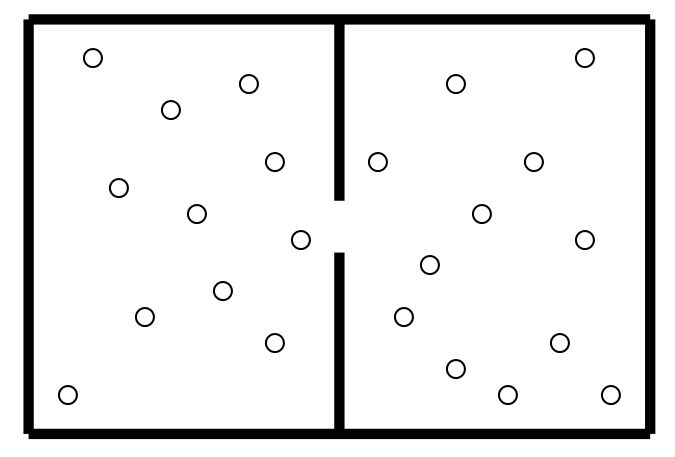
\includegraphics[width=0.5\textwidth]{Fig51.png}
\caption{(교재 5.1) Physical motivation for the Ehrenfest chain.}
\end{figure}

\paraorange{Example 5.1.3 Ehrenfest chain} 

$S=\{0,1,\dots,r\}$. 
\begin{align*}
& p(k,k+1)=(r-k)/r \\ 
& p(k,k-1)=k/r \\ 
& p(k,k+1)=0 \quad o.w.
\end{align*}
In words, there is a total of $r$ balls in two urns; $k$ in the first and $r-k$ in the second. We pick one of the $r$ balls at random and move it to the other urn. Ehrenfest used this to model the division of air molecules between two chambers (of equal size and shape) that are connected by a small
hole.

\paraviolet{해설} 에렌페스트의 체인도 마코프체인이다. 그리고 이것은 시간이 무한대로 가면 어떠한 상태로 수렴해 있을것이란 기대감이 있다. 즉 \textbf{이퀼리브리움(equilibrium)}으로 수렴할 것이란 기대감이 있는 마코프체인이다. 노드수가 유한개라면 이퀼리브리움으로 수렴하기 매우 유리하다는 사실을 눈치채면 좋겠다.에렌페스트 체인의 경우는 노드수가 $r$이다. 하지만 예제 5.1.2이나 예제 5.1.3은 노드수가 유한하지 않다. 

\paraorange{Example 5.1.4 Wright-Fisher model} 
Thinking of a population of $N/2$ dip-loid\footnote{디플로이드, 2배체의, 배수체의} individuals who have two copies of each of their chromosomes\footnote{크로모솜, 염색체} or of $N$ haploid\footnote{하프로이드, 반수체?} individuals who have one copy, we consider a
fixed population of $N$ genes that can be one of two types: $A$ or $a$. In the
simplest version of this model the population at time $n+1$ is obtained by
drawing with replacement from the population at time $n$. In this case,
if we let $X_n$ be the number of $A$ alleles\footnote{어리얼, 대립 형질[유전자]} at time $n$, then $X_n$ is a Markov chain with transition probability
\[
p(i,j)=\binom{N}{j}\left(\frac{i}{N}\right)^{j}\left(1-\frac{i}{N}\right)^{N-j}
\]
since the right-hand side is the binomial distribution for $N$ independent
trials with success probability $i/N$.

In this model the states $x = 0$ and $N$ that correspond to fixation of
the population in the all $a$ or all $A$ states are \textbf{absorbing states}\footnote{애브졸빙, 몰입하게 만드는}, that
is, $p(x, x) = 1$. As we will see this chain will eventually end up in state
$0$ or state $N$ . To make this simple model more interesting, we introduce mutations. That is, an $A$ that is drawn ends up being an a in the next
generation with probability $u$, while an $a$ that is drawn ends up being an
$A$ in the next generation with probability $v$. In this case the probability an $A$ is produced by a given draw is
\[
\rho_i=\frac{i}{N}(1-u)+\frac{N-i}{N}v
\]
but the transition probability still has the binomial form
\[
p(i,j)=\binom{N}{j}(\rho_i)^j(1-\rho_i)^{N-j}
\]
If $u$ and $v$ are both positive, then $0$ and $N$ are no longer absorbing states, so the system can converge to an equilibrium distribution as time $t \to \infty$?

\paraviolet{해설} 무슨말인지 잘 모르겠지만 총 $N$개의 노드가 있고 노드 $i$에서 $j$로 갈확률은 성공확률이 $\frac{i}{N}$인 시행에서 $j$번 성공하는 확률과 같다는 것이다. 

\paraorange{Example 5.1.5 M/G/1 queue} In this model, customers arrive according to a Poisson process with rate $\lambda$. ($M$ is for Markov and refers
to the fact that in a Poisson process the number of arrivals in disjoint
time intervals is independent.) Each customer requires an independent
amount of service with distribution $F$ . ($G$ is for general service distribution. $1$ indicates that there is one server.) Let $X_n$ be the number of customers waiting in the queue at the time the $n$th customer enters service. To be precise, when $X_0 = x$, the chain starts with $x$ people waiting in line and customer $0$ just beginning her service. To understand the definition the picture in Figure 5.2 is useful:

\begin{figure}[ht]
\center
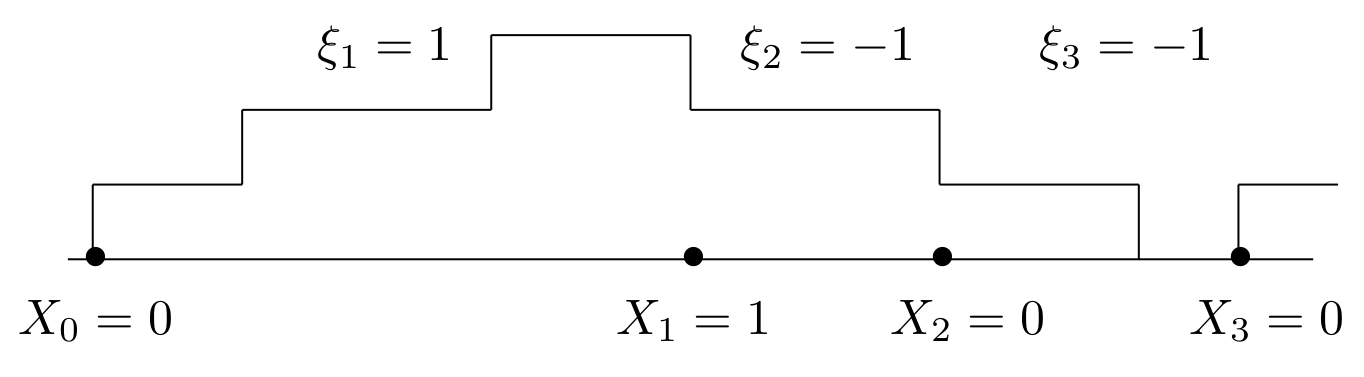
\includegraphics[width=0.7\textwidth]{Fig52.png}
\caption{(교재 5.2) Realization of the M/G/1 queue. Black dots indicate the times at which the customers enter service.}
\end{figure}

To define our Markov chain $X_n$ , let 
\[
a_k=\int_0^{\infty}e^{-\lambda t }\frac{(\lambda t)^k}{k!}dF(t)
\]

be the probability that $k$ customers arrive during a service time. Let
$\xi_1,\xi_2,\dots$ be i.i.d. with $P(\xi_i = k - 1) = a_k$ . We think of $\xi_i$ as the net number of customers to arrive during the ith service time, subtracting one for the customer who completed service. We define $X_n$ by
\[
X_{n+1}=(X_n+\xi_{n+1})^+ \quad \cdots (\star)
\]
The positive part only takes effect when $X_n = 0$ and $\xi_{n+1} = -1$ (e.g., $X_2 = 0, \xi_3 = −1$ in Figure 5.2) and reflects the fact that when the queue has size $0$ and no one arrives during the service time the next queue size is $0$, since we do not start counting until the next customer arrives and then the queue length will be $0$. 
It is easy to see that the sequence defined in $(\star)$ is a Markov chain
with transition probability
\begin{align*}
& p(0,0)=a_0+a_1 \\ 
& p(j,j-1+k)=a_k \quad \mbox{if}~~ j\geq1 \mbox{ or } k>1
\end{align*}
The formula for $a_k$ is rather complicated, and its exact form is not im-
portant, so we will simplify things by assuming only that $a_k > 0$ for all $k \geq 0$ and $\sum_{k\geq 0}a_k = 1$. 

\paraviolet{해설} 쉽게 생각하면 이런것이다. 은행에서 종업원앞에 있는 대기인원의 수를 $X_n$이라고 하자. 한번의 스텝은 종업원이 1명분의 일을 마쳤을때 이다. 즉 $X_0$는 최초대기인원의 수를 의미하고 $X_1$은 종업원이 첫고객을 응대한뒤 시점에서 카운트한 대기인원의 수이다. $n$이 $1$씩 증가함에 따라서 $X_n$이 평균 1.1씩 증가한다고 하자. 여기에서 각 노드들은 대기인원의 수를 의미하게 된다. 즉 $S=\{0,1,2,\dots,\}$이 되고 $X_n=5$라는것은 $X_n$이 5번노드에 있다는 것을 의미하고 $n$시점에서 종업원앞에 서있는 사람의 수가 5명이라는 의미가 된다. 

\dash

\subsection{Markov Property}
\paraorange{본문} If $X_n$ is a Markov chain with transition probability $p$, then by definition, 
\[
P(X_n \in B |{\cal F}_n)=p(X_n,B)
\]
In this section, we will prove two extensions of the last equality in which
$\{X_{n+1} \in B\}$ is replaced by a bounded function of the future, $h(X_n,X_{n+1},...)$, and $n$ is replaced by a stopping time $N$. These results, especially the second, will be the keys to developing the theory of Markov chains. As mentioned in previous Section, we can and will suppose that the $X_n$ are the coordinate maps on sequence space
\[
(\Omega_o,{\cal F}_{\infty})=\Big(S^{\{0,1,\dots\}},{\cal S}^{\{0,1,\dots\}}\Big)
\]
${\cal F}_n = \sigma(X_0, X_1,..., X_n)$, and for each initial distribution $\mu$ we have a measure $P_{\mu}$ defined by
\begin{align*}
& P(X_j\in B_j, 0\leq j\leq n)\\
&=\int_{B_0}\mu(dx_0)\int_{B_1}p_0(x_0,dx_1)\dots\int_{B_n}p_{n-1}(x_{n-1},dx_n)
\end{align*}
that makes $X_n$ a Markov chain with $P_{\mu}(X_0\in A) = \mu(A)$. Define the shift operators $\theta_n:\Omega_o,\to \Omega_o$ by 
\[
\theta_n(\omega_0,\omega_1,\dots)=(\omega_n,\omega_{n+1},\dots).
\]

\paraviolet{해설} 이번절에서는 아래의 정의를 확장하는 것에 대하여 다룬다. 
\[
P(X_n \in B |{\cal F}_n)=p(X_n,B)
\]
{\bf 확장은 2가지 측면에서 이루어진다.} (1) $X_n$대신에 $h(X_n,X_{n+1},\dots)$를 대입해도 성립하게 한다.\footnote{여기에서 $h$는 bounded and measurable function} (2) $n$대신에 stopping time $N$을 대입하여도 성립하게 한다. 이중에서 첫번째확장은 아래의 정리 5.2.3에의해서 성립한다. 이때 $Y=h(X_n,X_{n+1},\dots)$로 생각하면 된다. 

\paraorange{Theorem 5.2.3. The Markov property (첫번째확장)} Let $Y :\Omega_o\to \mathbb{R}$ be bounded and measurable.
\[
E_{\mu}\left(Y \circ \theta_m|{\cal F}_m \right)= E_{X_m} Y.
\]

\para{Remark} We denote the function by $Y$, a letter usually used for random variables, because that’s exactly what $Y$ is, a measurable function defined on our probability space $\Omega_o$. Here the subscript μ on the left-hand side indicates that the conditional expectation is taken with respect to $P_{\mu}$. The right-hand side is the function $\varphi(x)=E_xY$ evaluated at $x = X_m$.

\paraviolet{해설} (1) 우선 노테이션에 익숙해지는 연습을 하자. $Y$가 정의된 곳이 $\Omega_o$임을 주목하면 $Y$는 어떠한 \emph{path} $\bs{\omega}^*$를 실수값으로 맵핑하는 함수임을 알 수 있다. 예를들면 이런식이다. 
\[
Y(\bs{\omega}^*)=Y(\omega_0^*,\omega_1^*,\dots)=83.814
\] 
여기에서 $\bs{\omega}^* \in \Omega\times \Omega \times\dots$이고 $\omega_0^*\in \Omega=\{\tt node1, \dots, node24\}$임을 유의하자. 예를들어서 
\[
\omega_0^*={\tt node1}, ~~ \omega_1^*={\tt node20}, \dots 
\]
와 같다면 이 걸음열은 $\tt node1~ \to~ node20 ~\to ~ \dots$와 같이 이동하는 걸음열이다. 이 걸음들\footnote{$\omega_0^*,\omega_1^*,\dots$}의 흔적을 모은것을 $\bs{\omega}^*=(\omega_0^*,\omega_1^*,\dots)$으로 표현할 수 있는데 이런 이유로 나는 $\bs{\omega}^*$를 \textcolor{blue}{\emph{path}}라고 부르겠다. 아무튼 $Y$는 path를 어떠한 실수값으로 맵핑하는 함수이다. 이 쓸모없어 보이는 함수는 생각보다 유용한데 예를들어 "무한번 걸었을때 {\tt node1}에 머문 비율\footnote{$\frac{\mbox{노드1에 머문걸음}}{\mbox{총걸음}}$}이 얼마인가?"와 같은 물음을 정의할 수 있다. (2) $Y$를 아래와 같이 정의하자. 
\[
Y(\bs{\omega})=\frac{{\tt sum}(\bs{\omega}~{\tt == 1})}{|\bs{\omega}|}=\mbox{{\tt node1}에 머문비율}
\]
이제 정리 5.2.3의 결과의 의미를 살펴보자. 즉 
\[
E_{\mu}\left(Y \circ \theta_m|{\cal F}_m \right)= E_{X_m} Y.
\]
의 의미를 살펴보자. 좌변의 의미는 "초기분포 $\mu$에서 만들어진 path를 $m$만큼 평행이동시킨뒤 $m$시점 이전까지의 정보 ${\cal F}_m$를 모두 준 상태에서 노드1에 평균적으로 머문 비율을 계산한값"을 의미한다. 우변의 의미는 "초기에 $X_m=x_m=\omega_m$ 노드에서 만들어진 path에서 노드1에 평균적으로 머문 비율을 계산한 값"을 의미한다. 따라서 정리 5.2.3의 의미는 $X_m=x_m$을 알고 있는 이상 $(X_0,\dots,X_m)$의 분포에 대한 아무런 정보는 미래를 예측하는데 아무런 필요가 없으며 이때 $X_m,X_{m+1},\dots$는 마치 초기상태가 $x_m$인 마코프체인처럼 생각할 수 있다는 것이다. (3) (remark) 더렛은 $Y$는 함수이지만 마치 랜덤변수인것처럼 표현한다고 언급하였다. 이는 $Y$가 measurable function 이므로 성립한다. 

\paraorange{Theorem 5.2.4. Chapman-Kolmogorov equation} As corollary of Theorem 5.2.3 we get 
\[
P_x(X_{m+n}=z)=\sum_yP_x(X_m=y)P_y(X_n=z)
\]
Intuitively, in order to go from $x$ to $z$ in $m + n$ steps we have to be at some $y$ at time $m$ and the Markov property implies that for a given $y$ the two parts of the journey \footnote{저니, 여행. 즉 $x$는 출발노드 $z$는 도착노드이고 걸음은 여행, 즉 저니로 생각했다. $y$은 $m$걸음이후 도착한 경유지이다. 이 여행은 $x$에서 출발하고 $m$걸음 이후에 $y$에 도착하고 $m+n$걸음 이후에 $z$로 도착하게 된다.} are independent.

\proof $P_x(X_{n+m}=z)=E_x(P_x(X_{n+m}=z|{\cal F}_m))=E_x(P_{X_m}(X_n=z))$ by the Markov property, Theorem 5.2.3 since $1_{(X_n=z)}\circ \theta_m=1_{(X_{n+m=z})}$. 

\paraorange{교재(두번째확장)} We are now ready for our second extension of the Markov property.
Recall $N$ is said to be a stopping time if $\{N = n\}\in {\cal F}_n$. As in Chapter Martingales, let
\[
{\cal F}_N=\{A:A\cap \{N=n\} \in {\cal F}_n \quad \mbox{for all } n\}
\]
be the information known at time $N$, and define the random shift operator
\[
\theta_N \omega = 
\begin{cases}
\theta_n \omega  & \quad \mbox{on}\quad \{N=n\} \\ 
\Delta  & \quad \mbox{on}\quad \{N=\infty\} \\ 
 \end{cases}
\]
where $\Delta$ is an extra point that we add to $\Omega_o$. In the next result and its applications, we will explicitly\footnote{익스플리시티, 명쾌하게} restrict our attention to $\{N<\infty\}$, so the reader does not have to worry about the second part of the definition of $\theta_N$.

\paraviolet{해설} 기호들을 정리하자. (1) 먼저 \textcolor{blue}{${\cal F}_N$}에 대하여 정리하자. 
\[
{\cal F}_N=\{A:A\cap \{N=n\} \in {\cal F}_n \quad \mbox{for all } n\}
\]
은 시점 $N$까지의 정보가 모두 모인 시그마필드이다. 이때 $A$는 무한열이 정의되는 공간 ${\cal F}_{\infty}$의 원소인 이벤트임에 주의하자. 즉 $A \in {\cal F}_{\infty}$이다. (2) 이제 쉬프트오퍼레이터 \textcolor{blue}{$\theta_n$}에 대하여 정의하자. 이는 $\omega\in {\Omega}_{o}$를 $n$번 이동시켰다는 의미가 된다. 이때 $\theta_n \omega$에서 언급된 $\omega$는 벡터이다. 따라서 오히려 $\bs{\omega}$로 표현하는것이 덜 헷갈릴 수도 있을것 같다. 아래를 관찰하자. 
\[
\theta_n \bs{\omega}=\theta_n (\omega_0,\omega_1,\dots )=(\omega_n,\omega_{n+1},\dots)
\]
(3) 이제 \textcolor{blue}{$N$}에 대하여 알아보자. $N$은 확률변수이다. 무한대의 값을 가질수도 있다. $N$으로 걸음열을 shift하는 상황을 생각해보자. 이를 위해서 교재에서는 random shifting operator $\theta_N$을 정의하였다. $N$이 어떤 유한한 값 $n$이라면 $\theta_N\omega=\theta_n\omega$라고 정의할 수 있다. 그런데 $N$이 무한한 값을 가진다면 어떻게 될까? 일단 이런경우에 관심은 없다. 우리는 $\{N<\infty\}$에만 관심이 있다. 하지만 $\{N=\infty\}$인 경우에도 정의를 하긴 해야하므로 이런 경우가 발생하는 event를 $\Delta$라고 정의하고 이 집합을 $\Omega_o$에 추가한다. (단지 정의를 깔끔하게 하기 위해서이다. 따라서 실제로는 $\{N=\infty\}$일 경우를 완전히 머리속에서 지워도 괜찮다.)

\paraorange{Theorem 5.2.5. Strong Markov property} 
Suppose that for each $n$, $Y_n : \Omega_o \to \mathbb{R}$ is measurable and $|Y_n|\leq M$ for all $n$. Then
\[
E_{\mu}(Y_N\circ\theta_N|{\cal F}_N)=E_{X_N}Y_N \quad \mbox{on}~ \{N<\infty\} 
\]
where the right-hand side is $\varphi(x,n) = E_xY_n$ evaluated at $x = X_N$, $n = N$.

\proof Let $A \in {\cal F}_N$. Breaking things down according to the value of $N$. 
\[
E_{\mu}(Y_N\circ \theta_N ; A \cap \{N<\infty\})=\sum_{n=0}^{\infty}E_{\mu}(Y_n\circ \theta_n; A\cap \{N=n\})
\]
Since $A\cap \{N=n\} \in {\cal F}_n$, using Theorem 5.2.3 now converts the right side into 
\[
\sum_{n=0}^{\infty}E_{\mu}(E_{X_n}Y_n; A\cap \{N=n\})=E_{\mu}(E_{X_N}Y_N; A\cap \{N<\infty\})
\]

\para{Remark} The reader should notice that the proof is trivial. All we do is break things down according to the value of $N$ , replace $N$ by $n$, apply the Markov property, and reverse the process. This is the standard technique for proving results about stopping times. 

\paraviolet{해설} (1) (2) 증명과정을 살펴보자. 우선 
\[
A \in {\cal F}_N \Longleftrightarrow A \cap \{N=n\} \in {\cal F}_n \quad \mbox{for all $n$.}
\]
임을 기억하자. 그리고 아래등호가 성립하는 이유를 알아보자. 
\[
E_{\mu}(Y_N\circ \theta_N ; A \cap \{N<\infty\})=\sum_{n=0}^{\infty}E_{\mu}(Y_n\circ \theta_n; A\cap \{N=n\})
\]
$\{N=\infty\}=\emptyset$을 가정하면 아래와 같이 표현할 수 있다. 
\[
A\cup\{N<\infty\}=A\cup\big(\bigcup_{n=1}^{\infty}\{N=n\}-\{N=\infty\}\big)
\]


\paraorange{본문} Our first application of the strong Markov property will be the key to
developments in the next section. Let $T_y^0 = 0$, and for $k\geq 1$, let
\[
T_y^k=\inf \left\{n>T_y^{k-1}: X_n=y\right\}.
\]
$T_y^k$ is the time of $k$-th return to $y$. The reader should note that $T_y^1>0$ so any visit at time $0$ does not count. We adopt this convention so that if we let $T_y=T_y^1$ and $\rho_{xy}=P_x(T_y<\infty)$, then 

\para{Theorem 5.2.6}
$P_x(T_y^k<\infty)=\rho_{xy}\rho_{yy}^{k-1}$

\bk Intuitively, in order to make $k$ visits to $y$, we first have to go 
from $x$ to $y$ and then return $k-1$ times to $y$. 

\paraviolet{해설} (1) \textcolor{blue}{$T_y^k$}는 노드 $y$를 $k-1$번째 방문한상태에서, $k$번째 방문하기 위해 진행해야할 \textbf{걸음수}를 표현하는 개념이다. 어떠한 사람이 상태 $y$를 24걸음만에 첫방문하고, 그다음은 38걸음에서, 그다음은 50걸음에서 방문하였다고 하자. 그러면 $T_y^1=24, T_y^2=38, T_y^3=50$이 된다. (2) 따라서 $T_y^{\textcolor{orange}{1}}=\textcolor{violet}{0}$ 라는 의미는 노드 $y$를 \textcolor{violet}{0}걸음만에 첫 방문(\textcolor{orange}{1}번째 방문) 할 수 없다는 말이다. $0$걸음만에 방문한다는 것은 처음부터 $y$에 있었다는 의미이다. 초기분포는 $P_x$에서 결정되어야 할 사항이므로 여기에서는 이런 경우를 제외해야 합리적일것 같다. 그래서 제외한다. 즉 $T_y^{\textcolor{orange}{1}}>\textcolor{violet}{0}$ 을 가정한다. (3) \textcolor{blue}{$T_y=T_y^1$}와 같이 약속한다. (4) {$\rho_{xy}=P_x(T_y<\infty)$}의 의미를 알아보자. 그전에 $T_y<\infty$의 의미를 알아보자. 우선 $T_y=T_y^1$는 노드 $y$를 최초 1번 방문하기 위해 필요한 걸음수이다. 따라서 $T_y=\infty$라는 것은 "노드 $y$를 방문할 수 없다"는 의미가 된다. 동일한 논리로 $T_y<\infty$라는 것은 "언젠가 노드 $y$를 방문할 수 있다"는 의미가 된다. 따라서 \textcolor{blue}{$\rho_{xy}$}는 노드 $x$에서 시작하여 노드 $y$를 언젠가 방문할 확률을 의미한다. 즉 $\rho_{xy}>0$이라는 의미는 "노드$x$에서 시작하여 노드$y$를 언젠가 방문할 확률이 $0$은 아님"을 의미하고 이말은 "노드 $x$와 노드 $y$가 \textcolor{blue}{연결}"되었다는 의미가 된다. (4) 따라서 정리 5.2.6의 의미는 아래와 같다. 
\begin{itemize}
	\item 좌변 = $P_x(T_y^k<\infty)$ = $x$에서 출발하여 $y$를 $k$번 방문할 확률
	\item 우변 = $\rho_{xy}\rho_{yy}^{k-1}$ = ($x$에서 출발하여 $y$를 1번 방문할 확률) $\times$ ($y$에서 출발하여 $y$를 $k-1$번 방문할 확률)
\end{itemize}

\paraorange{본문} The next example illustrates the use of Theorem 5.2.5, and explains why we want to allow the $Y$ that we apply to the shifted path to depend on $n$. 

\paraviolet{해설} 아래의 정리는 왜 $X_n$이 아니라 $Y_n$에 관심을 가지면 좋은지에 대한 설명을 해준다. (??)

\paraorange{Theorem 5.2.7. Reflection principle} Let $\xi_1,\xi_2,\dots$ be independent and identically distributed with a distribution that is symmetric about $0$. Let $S_n=\xi_1+\dots+\xi_n$. If $a > 0$ then
\[
P\left(\sup_{m\leq n} S_m \leq a\right) \leq 2P(S_n \geq a)
\]
We do the proof in two steps because that is how formulas like this are
derived in practice. First, one computes intuitively and then figures out
how to extract the desired formula from Theorem 5.2.5.

\para{Proof in words} First note that if $Z$ has a distribution that is symmetric about $0$, then
\[
P(Z \geq 0) \geq P(Z>0) + \frac{1}{2}P(Z = 0) =\frac{1}{2}
\]
If we let $N = \inf\{m \leq n : S_m > a\}$ (with $\inf\emptyset = \infty$), then on $\{N < \infty\}$, $S_n - S_N$ is independent of $S_N$ and has $P(S_n - S_N \geq 0) \geq \frac{1}{2}$ So
\[
P(S_n>a)\geq \frac{1}{2}P(N\leq n)
\]

\paraviolet{해설} (1) 우선 정리 5.2.7을 간단히 살펴보자. $\xi_i$를 무기억과정 혹은 백색잡음과정이라고 부른다. 따라서 $S_n$은 무기억과정의 누적합 혹은 백색잡음과정의 누적합이 된다. 간단하게 이를 \textcolor{blue}{\bf 잡음합}으로 부르자.\footnote{나만 쓰는 용어다} $S_n$이 걸음열임은 쉽게 알 수 있다. 그리고 일반적으로 잡음합은 항상 걸음열이 된다. 정리 5.2.7의 의미를 알아보자. 좌변 즉 $P\left(\sup_{m\leq n} S_m \leq a\right)$의 의미는 $n$이라는 제한된 시행횟수 속에서 걸음합 $S_m$이 한번도 $a$를 넘지못할 확률을 의미한다. 우변 $P(S_n\geq a)$의 의미는 $n$시점에서 걸음합이 $a$를 넘어서있을 확률을 의미한다. 좌변의 확률은 계산하기 어렵지만 우변의 확률은 상대적으로 계산하기 쉬우므로 이 부등식은 유용하다. (2) 좀더 쉽게 예제와 함께 설명하면 이런것이다. 랜덤으로 오른쪽 왼쪽 걸어서 움직인다고 하자. 우연히 걷다가 $(1,0)$의 위치에 가면 회사에 출근해야 한다고 하자. $n=3$이라고 하면 회사에 출근하는 경우는 $\rightarrow, ?, ? $와 $\leftarrow, \rightarrow, \rightarrow$ 이므로 확률은 $\frac{1}{2}+\frac{1}{8}=\frac{5}{8}$이다. 따라서 출근안할 확률은 $P(\sup_{m\leq 3}S_m\leq 0)=\frac{3}{8}$이다. 그런데 $P(S_3\geq 0)=\frac{1}{2}$ 이다. (2) $N$의 의미가 궁금하다. 그런데 $N$의 의미를 알아보기 전에 $N$이 stopping time임을 체크해보자. $N=\inf\{m\leq n:S_m>a\}$에서 $m\leq n$이라는 조건 때문에 $N$은 stopping time이 된다. (3) \textcolor{blue}{$N$의 의미:} 걸음을 $n$번 걸었다고 하자. $m\leq n$에 대하여 $S_m>a$이 되는 첫시점을 $N$이라고 정의한다. 만약에 $n$번째 걸음 이전에 $S_n>a$가 달성되지 못하면 $\{m\leq n:S_m>a\}=\emptyset$이 되는데 이 경우는 $N=\infty$로 정의한다. \footnote{왜냐하면 $\inf \emptyset=\infty$라고 하였으므로} 즉 다시한번 요약하면 {\bf $N$은 \textcolor{blue}{잡음합}이 처음으로 $a$보다 크게 되는 시점을 의미한다.} 만약에 \textcolor{blue}{잡음합}이 $n$시점 이전에 $a$를 넘긴적이 없다면 $N=\infty$로 정의한다는 의미이다. (4) 이제 증명과정을 찬찬히 살펴보자. 증명의 꽃은 $N$이 stopping time임을 이용하여 사용하는 테크닉이다. 이 테크닉때문에 이 정리를 살펴보았다. 먼저 
\[
S_n-S_N=\xi_{N+1}+\dots+\xi_{n}
\]
와 같이 둘 수 있음을 관찰하자.  여기에서 $\xi_{N+1},\xi_{N+2},\dots,\xi_n$는 각각 i.i.d. and symmetric about $0$인 분포를 가지므로 
$
P(S_n-S_N\geq 0) \geq  \frac{1}{2}
$
이다. 그런데 
\begin{align*}
& \big\{S_n > a\big\}=\big\{S_N > a, \mbox{ and } S_n-S_N \geq 0 \big\}  \\ 
& =\textcolor{red}{\big\{S_N > a \big\}} \cap\big\{ S_n-S_N \geq 0 \big\} \\
&= \textcolor{red}{\big\{N\leq n\big\}}\cap \big\{ S_n-S_N \geq 0 \big\} \quad \cdots (\star)
\end{align*}
로 표현가능하다. 두번째 등호는 $S_N$과 $S_n-S_N$이 독립임을 이용하였다. 세번째 등호는  빨간부분 즉 $\{S_N>a\}=\{N\leq n\}$임을 이용했는데 이 부분이 바로 증명의 꽃이며 stopping time을 쓰는 이유이다. 아무튼 $(\star)$에서 확률메저 $P$를 취하면 
\[
P(S_n>a) = P(N\leq n) P(S_n-S_N \geq 0)
\]
이 된다. 그런데 $P(S_n-S_N \geq 0)\geq \frac{1}{2}$이므로 아래가 성립한다. 
\[
P(S_n>a)\geq \frac{1}{2}P(N\leq n) \quad \Leftrightarrow \quad 2P(S_n>a)\geq P(N\leq n)
\] 
그런데 여기에서 $\{N\leq n\}=\{S_N>a\}=\Big\{\underset{m\leq n}{\sup}S_m>a\Big\}$ 이므로 원하는 것이 증명된다. 

\paraorange{More formal proof of Thm 5.2.7} Let $Y_m(\omega) = 1$ if $m \leq n$ and $\omega_{n-m}\leq a$, $Y_m(\omega) = 0$ otherwise. The definition of $Y_m$ is chosen so that $(Y_N \circ \theta_N)(\omega) = 1$ if $\omega_n\geq a$ (and
hence $N \leq n$), and $= 0$ otherwise. The strong Markov property implies
\[
E_0(Y_N \circ \theta_N |{\cal F}_N) = E_{S_N} Y_N \quad \mbox{on}~\{N<\infty\} = \{N\leq n\}
\]
To evaluate the right-hand side, we note that if $y > a$, then
\[
E_yY_m=P_y(S_{n-m}\leq a)\leq P_y(S_{n-m}\leq y)\leq \frac{1}{2}
\]
So integrating over $\{N \leq n\}$ and using the definition of conditional
expectation gives
\[
\frac{1}{2}P(N \leq n) \leq  E_0\big(E_0 (Y_N \circ \theta_N | {\cal F}_N); N \leq n\big) = E_0 (Y_N \circ \theta_N ; N \leq n)
\]
since $\{N \leq n\} \in {\cal F}_N$. Recalling that $Y_N \circ \theta_N = 1_{\{S_n \leq a\}}$, the last quantity 
\[
= E_0(1_{\{S_n \geq a\}}; N \leq n) = P_0 (S_n \geq a)
\]
since $\{S_n > a\} \subset \{N \leq n\}$.

\dash

\subsection{Recurrence and Transience}
\paraorange{본문(리커런트,트렌지언트)} Let $T_y^0=0$, and for $k\geq q$, let
\[
T_y^k=\inf\{n>T_y^{k-1}: X_n=y\}
\]
and recall Theorem 5.2.6
\[
\rho_{xy}=P_x(T_y<\infty). 
\]
(See more detail explanation\footnote{$\rho_{xy}=P_x(T_y<\infty)$인 이유를 알아보자. 정리 5.2.6에 의하면 
\[
P_x(T_y^k<\infty)=\rho_{xy}\rho_{yy}^{k-1}
\]
이다. 여기에서 $k=1$을 대입하면 $\rho_{xy}=P_x(T_y^1<\infty)=P_x(T_y<\infty)$를 얻는다. 두번때 등호는 $T_y^0=0$이라고 가정하였으므로 성립한다.}) A state $y$ is said to be \textcolor{blue}{\bf recurrent}\footnote{되풀이되는} if $\rho_{yy}=1$ and \textcolor{blue}{\bf transient}\footnote{일시적인} if $\rho_{yy}<1$. 

\paraviolet{해설} $\rho_{xy}$의 뜻은 걸음열이 $x$에서 출발하여 언젠가 한번은 $y$를 방문할 확률을 의미한다. 동일한 논리로 $\rho_{yy}$의 뜻은 걸음열이 $y$에서 출발하여 언젠가 한번은 다시 $y$를 방문할 확률을 의미한다. 만약에 $\rho_{yy}=1$이라면 이 걸음열은 $y$를 \textcolor{blue}{계속하여 반복적으로} 방문하게 된다. 만약에 $\rho_{yy}<1$이라면 걸음열은 $y$에 \textcolor{blue}{일시적으로만} 있다. {\bf 좀 더 구체적인 설명을 위하여 친숙한 예제를 들어보자.} 노드들을 어떠한 회사라고 하자. 근로자는 1년단위로 회사와 재계약을 한다. 근로자가 회사를 옮기는 과정을 "걸음"이라고 이해하자. 어떠한 회사 $y$에 대하여 $\rho_{yy}=1$이라는 의미는 근로자가 $y$라는 회사에 한번 근무하면 언젠가 다시 $y$회사에 재근무할 확률이 100\%라는 것을 의미한다.\footnote{언젠가 다시 근무한다는 것이지 매년 그 회사에서 근무한다는 의미는 아니다. 즉 어떤 근로자가 노드 $x$에서 1년 노드 $y$에서 1년 다시 노드$x$에서 1년 $\dots$와 같은식으로 근무를 반복해도 $\rho_{yy}=1$이다.} 만약에 $\rho_{yy}<1$라면 그 회사에 계속하여 반복적으로 근무함을 보장할 수는 없다는 것을 의미한다.\footnote{이것도 그 회사와 언젠가 떠난다는 것을 의미하는 것은 아니다. 운이 좋으면 다시 근무할 수 있다는 의미같음.} 

\note 모든 상태는 리커런트하거나 트랜지언트 하다. (정의를 읽어보자.)

\paraorange{본문} If $y$ is recurrent, Theorem 5.2.6\footnote{$P_x(T_y^{k}<\infty)=\rho_{xy}\rho_{yy}^{k-1}$} implies $P_y(T_y^k < \infty) = 1$ for all $k$, so $P_y(X_n = y~ i.o.) = 1$.
If $y$ is transient and we let $N(y)=\sum_{n=1}^{\infty} 1_{(X_n=y)}$ be the number of visits to $y$ at positive times, then 
\begin{align*}
&E_xN(y)=\sum_{k=1}^{\infty}P_x(N(y)\geq k)=\sum_{k=1}^{\infty}P_x(T_y^k<\infty)\\ 
&=\sum_{k=1}^{\infty}\rho_{xy}\rho_{yy}^{k-1}=\frac{\rho_{xy}}{1-\rho_{yy}}<\infty
\end{align*}
Combining the last computation with our result for recurrent states gives
\para{Theorem 5.3.1} $y$ is recurrent if and only if $E_yN(y)=\infty$.

\bk The next result shows that recurrence is contagious.\footnote{콘테이져스, 전염되는}

\para{Theorem 5.3.2} If $x$ is recurrent and $\rho_{xy}>0$ then $y$ is recurrent and $\rho_{yx}=1$. 

\paraviolet{해설} (1) Theorem 5.3.1을 설명해보자. $N(y)$의 의미는 $y$라는 회사에서 근무한 횟수를 의미한다. 만약에 $y$가 반복해서 근무할만한 회사라면, 즉 state $y$가 리커런트하다면 $N(y)=\infty$이다. 이 내용이 정리 5.3.1의 내용이다. 정리 5.3.1 에서는 $E_yN(y)=\infty$라고 되어있는데 이는 그냥 출발점이 $y$라는 것을 다시 명시한 효과이다.\footnote{회사가 2개의 그룹으로 되어있다고 하자. 예를들어 IT회사와 제조업회사. 두 그룹은 서로 연결되어 있지 않다고 하자. 즉 IT계열에 근무한 사람은 계속 IT계열로만 이직하고 반대도 마찬가지이다. $y$는 IT회사에 속한다고 하자. $y$가 아무리 리커런트해도 최초에 근로자가 제조업계열로 근무했다면 $N(y)=0$이다. 따라서 리커런트한 state를 표현하기 위해서는 $N(y)$로만 활용하면 부족하고 출발점을 명시하는 개념이 필요하다.} (2) 이제 Theorem 5.3.2의 내용을 설명해보자. 요약하면 리커런트한 상태는 전염성이 있다는 말이다. 이게 무슨뜻일까? 만약에 상태 $x$가 리커런트하고 상태 $x$에서 $y$로 갈 확률이 0이 아니라면 $y$도 리커런트하다. 왜냐하면 어차피 $x$에서는 무한번 근무할 것이고 $x$에서 $y$로 갈확률이 0이 아니라면 $y$에서도 근무할 것이기 때문이다. 그 비율은 대충 
\[
\frac{\mbox{$y$에서 근무한횟수}}{\mbox{$x$에서 근무한횟수}}\approx \rho_{xy}
\]
일텐데 $x$에서 무한번 근무하므로 $y$에서도 무한번 근무하게 된다. 또한 $x$에서 근무하고 $y$로 왔다면 반드시 다시 언젠가는 $x$에서 근무하게 되어있으므로 (왜냐하면 $x$가 리커런트하니까) $\rho_{yx}=1$이다. 이것이 정리 5.3.2의 내용이다. 

\paraorange{본문(closed,irreducible)} The next fact will help us identify recurrent states in examples. First
we need two definitions. $C$ is \textcolor{blue}{\bf{closed}} if $x \in C$ and $\rho_{xy}>0$ implies $y \in C$. The name comes from the fact that if $C$ is closed and $x \in C$ then $P_x(X_n\in C)=1$ for all $n$. $D$ is \textcolor{blue}{\bf{irreducible}} if $x, y \in D$ implies $\rho_{xy} > 0$.

\paraviolet{해설} (1) closed는 \textcolor{blue}{"탈출불가능"}의 의미이다. 어떤 노드들의 집합 $C$가 closed라는 의미는 $C$안의 임의의 노드에서 시작한 걸음은 반드시 그 도착점이 $C$내에만 있어야 한다는 의미이다. (2) irreducible은 번역그대로 하면 \textcolor{blue}{"축소불가능한"}이지만, 수식을 보면
\textcolor{blue}{"서로(쌍방) 도달가능한"}의 의미이다. 쌍방도달가능하다는 것은 서로 연결\footnote{\textcolor{red}{완전 직접적으로 연결되어있지 않더라도!! 즉 링형태의 그래프는 모두 연결은 되어있지만 모든 노드가 직접적으로 연결되어있는 것은 아님}} 되어있다는 의미이므로 어떤 문헌에서는 \textcolor{blue}{"연결가능한"}의 의미로 쓰이기도 한다.\footnote{그래서 교재에 따라서는 \textcolor{blue}{{\bf irreducible}} 대신에 \textcolor{blue}{{\bf strongly connected}} 라는 말을 쓰기도 한다.} 어떤 노드들의 집합 $D$가 irreducible하다는 것은 $D$에 속하는 어떠한 두 노드 $x,y$에 대하여 $\rho_{xy}>0$ 이면서 동시에 $\rho_{yx}>0$임을 의미한다. (3) 참고로 원래 어떠한 노드들의 집합에 대하여 이리듀시블하다고 말는 것이 정의이지만 transition probability에 대하여 이리듀시블 하다고 표현하기도 한다. 즉 \textcolor{blue}{$p$가 이리듀시블하다}와 같은 식으로 말이다. 이리듀시블은 집합 $D$의 어떤 성질을 표현하는 말이지만 그 성질은 전이확률 $p$로 정의되기 때문에 \textbf{suppose $p$ is irreducible}과 표현들을 혼용하여 사용한다. 이러한 정의는 Theorem 5.5.6에서 처음 등장한다. 

\paraorange{Theorem 5.3.3} Let $C$ be a finite closed set. Then $C$ contains a recurrent state. If $C$ is irreducible then all states in $C$ are recurrent.

\paraviolet{해설} (1) \textcolor{gray}{\emph{"Let $C$ be a finite closed set. Then $C$ contains a recurrent state."}} 이 무슨뜻일까? 이런경우가 가능한 예를들어보자. 2개의 노드로 이루어진 집합 $C$를 생각하고 노드1에서 노드2로가는 화살표만 있다고 가정하자. 걸음열은 집합 $C$를 \textcolor{blue}{\bf "탈출할 수 없으므로"} $C$는 클로즈드이다. 결국에는 노드2에서만 머물게 되므로 노드2는 리커런트 스테이드이다. \footnote{참고로 이때 노드2와 같은 state를 \textcolor{blue}{\textbf{absorbing state}}라고 한다. 예제 5.3.6을 참고하라.} (2) 그렇다면 \textcolor{gray}{\emph{"If $C$ is irreducible then all states in $C$ are recurrent."}}의 상황을 표현하는 예제는 무엇인가? 아까의 예제에서 이제 노드2에서 노드1로 가는 화살표가 추가된다고 가정해보자. 집합 $C$의 모든 노드들은 \textcolor{blue}{\bf "서로(쌍방) 도달 가능"}하다. 즉 노드1에서 노드2로 갈수있고 노드2에서도 노드1로 갈수 있다. 따라서 집합 $C$는 이리듀시블하다. 이때는 노드1에서 절반정도 노드2에서 절반정도 걸음열이 머물며 이 상태가 무한번 일어나므로 노드1,2모두 리커런트 스테이트가 된다. 

\paraorange{Example 5.3.4 A Seven-state chain} Consider the transition probability:
\begin{figure}[ht]
\center
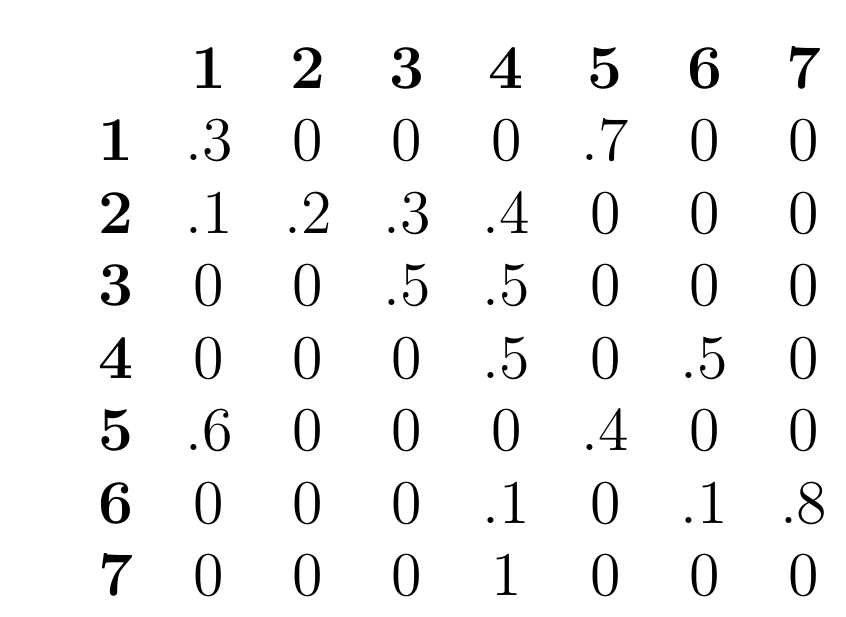
\includegraphics[width=0.5\textwidth]{Ex534table.png}
\caption{(교재에 소개된 테이블) A Seven-state chain.}
\end{figure}
To identify the states that are recurrent and those that are transient, we
begin by drawing a graph that will contain an arc from $i$ to $j$ if $p(i, j) > 0$ and $i \neq j$. We do not worry about drawing the self-loops corresponding to states with $p(i, i) > 0$ since such transitions cannot help the chain get somewhere new.
In the case under consideration we draw arcs from $\tt 1 \to 5$, $\tt 2 \to 1$, $\tt 2 \to 3$, $\tt 2 \to 4$, $\tt 3 \to 4$, $\tt 4 \to 6$, $\tt 4 \to 7$, $\tt 5 \to 1$, $\tt 6 \to 4$, $\tt 6 \to 7$, $\tt 7 \to 4$.
\begin{figure}[ht]
\center
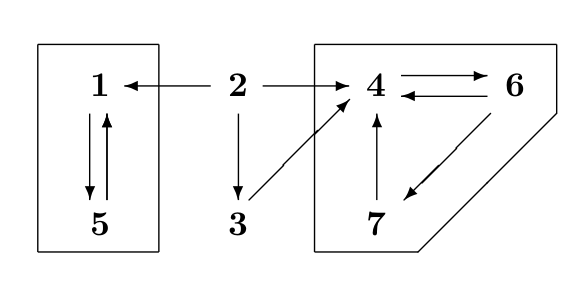
\includegraphics[width=0.5\textwidth]{Fig54.png}
\caption{(교재 5.4) Graph for the seven state chain.}
\end{figure}
\begin{enumerate}[(i)]
\item $\rho_{21}>0$ and $\rho_{12}=0$ so $\tt 2$ must be transient, or we would contradict Theorem 5.3.2. Similarly, $\rho_{34} > 0$ and $\rho_{43}=0$ so $\tt 3$ must be transient.
\item $\tt \{1, 5\}$ and $\tt \{4, 6, 7\}$ are irreducible closed sets, so Theorem 5.3.3 implies these states are recurrent.
\end{enumerate}
The last reasoning can be used to identify transient and recurrent
states when $S$ is finite since for $x \in S$ either: (i) there is a $y$ with $\rho_{xy}> 0$ and $\rho_{yx}=0$ and $x$ must be transient, or (ii) $\rho_{xy}>0$ implies $\rho_{yx}>0$. In case (ii), Exercise 5.3.2 \textcolor{red}{\bf($\rho_{xz}\geq \rho_{xy}\rho_{yz}$)} implies $C_x = \{y : \rho_{xy} > 0\}$ is an irreducible closed set. (If $y, z \in C_x$ then $\rho_{yx}\geq \rho_{yx}\rho_{xz}>0$. If $\rho_{yw}>0$ then
$\rho_{xw}\geq \rho_{xy}\rho_{yw}>0$, so $w \in C_x$.) So Theorem 5.3.3 implies $x$ is recurrent.

\paraviolet{해설} 유용한 예제. (1) 그림의 {\tt node 1, 5} / {\tt node 4,5,7} 은 리커런트한 노드이다. 그리고 {\tt node 2,3}은 트렌지언트한 노드이다. (2) $\tt \{1, 5\}$ and $\tt \{4, 6, 7\}$ 은 closed and irreducible set 이다. 

\paraorange{Theorem 5.3.5 Decomposition theorem} Let $R = \{x : \rho_{xx} = 1\}$ be the recurrent states of a Markov chain. $R$ can be written as $\cup_i R_i$, where each $R_i$ is closed and irreducible.

\para{Remark} This result shows that for the study of recurrent states we
can, without loss of generality, consider a single irreducible closed set.

\paraviolet{해설} 그러니까 결국 정리 5.3.5를 통해서 이런말을 하고 싶은것 같다. (1) 모든 노드들은 리커런트 하거나 트렌지언트 한 상태이다. (2) 이제 리커런트한 노드들만을 모아놓은 집합을 $R$이라고 하자. (3) 그런데 $R$은 정리 5.3.5에 의해서 closed and irreducible한 집합들의 합으로 분해할 수 있다. 즉 $R=\cup_{i}R_i$. (4) 따라서 리커런트한 상태의 노드들을 모은집합 $R$에 대하여 어떠한 성질들을 연구하는것은 closed and irreducible set $R_i$에 대한 성질을 연구하는 것과 동치이다. 

\paraorange{본문} The rest of this section is devoted to examples. Specifically we concentrate on the question: How do we tell whether a state is recurrent or
transient? Reasoning based on Theorem 5.3.2 works occasionally when $S$ is infinite.

\para{Example 5.3.6 Branching process} If the probability of no children
is positive then $\rho_{k0} > 0$ and $\rho_{0k}=0$ for $k \geq 1$, so Theorem 5.3.3 implies all states $k \geq 1$ are transient. The state $0$ has $p(0, 0) = 1$ and is recurrent. It is called an \textcolor{blue}{\bf absorbing state} to reflect the fact that once the chain enters $0$, it remains there for all time.

\bk If $S$ is infinite and irreducible, all that Theorem 5.3.2 tells us is that either all the states are recurrent or all are transient, and we are left to figure out which case occurs. \footnote{노드수가 무한이고 쌍방도달가능이면 모든 상태가 리커런트하거나 모든 상태가 트렌지언트 하다.}

\paraviolet{해설} 어떠한 노드가 리커런트한지 트랜지언트한지 어떻게 할수있을까? 본문에서는 이것이 {\bf 속도의 문제}라고 이야기하는것 같다. 즉 $n$이 커짐에 따라 갈수있는 노드수(=회사수)가 얼마나 빠르게 증가하느냐에 따라 달라진다. 즉 무한대로 터지는 {\bf 속도의 문제}이다. 어떤사람이 이직을 한다고 하자. $n$, 즉 이직횟수가 무한대로 증가함에 따라 갈수있는 회사가 점점 기하급수적으로 많아지는 사람은 모든회사가 그저 거쳐가는 회사(\textcolor{blue}{트렌지언트})일 것이다. 하지만 이직횟수가 무한대로 감에 따라 회사의 수가 매우 천천히 (그러나 무한대로) 증가하는 경우라면 모든 회사가 \textcolor{blue}{리커런트}한 회사이다. 

\paraorange{Example 5.3.7 M/G/1 queue} Let $\mu=\sum k a_k$ be the mean number of customers that arrive during one service time. 

\para{Remark} There is another way of seeing that the M/G/1 queue is
transient when $\mu>1$. If we consider the customers that arrive during a
person’s service time to be her children, then we get a branching process.
Results in Section 5.3 imply that when $\mu\leq 1$ the branching process dies out with probability one (i.e., the queue becomes empty), so the chain is recurrent. When $\mu>1$, Theorem 4.3.12 implies $P_x(T_0<\infty)=\rho^x$, where $\rho$ is the unique fixed point $\in (0,1)$ of the function $\varphi(\theta)=\sum_{k=0}^{\infty}a_j\theta^k$.

\paraorange{본문} The next result encapsulates\footnote{엔캡설레이트, 요약하다. 압축하다.} the techniques we used for birth and death chains and the M/G/1 queue. 

\para{Theorem 5.3.8} Suppose $S$ is irreducible, and $\varphi\geq 0$ with $E_x \varphi(X_1)\leq \varphi(x)$ for $x \notin F$, a finite set, and $\varphi(x)\to \infty$ as $x \to \infty$, i.e., $\{x : \varphi(x) \leq M \}$ is finite for any $M < \infty$, then the chain is recurrent.

\paraviolet{해설} 결국 정리 5.3.8도 {\bf 속도의문제}를 다루고 있는것 같다. 

\paraorange{Example 5.3.9. Birth and death chains on $\{0,1,2,...\}$} 나중에 공부하자.

\paraorange{Theorem 5.3.10} If $a<x<b$ then 
\[
P_x(T_a<T_b)=\frac{\varphi(b)-\varphi(x)}{\varphi(b)-\varphi(a)}, \quad P_x(T_b<T_a)=\frac{\varphi(x)-\varphi(a)}{\varphi(b)-\varphi(a)}
\]

\paraviolet{해설} 정리 5.3.10은 Birth and death chains에 한정하여 사용할 수 있는 정리이다. 여기에서 
\[
T_a=\inf \{n\geq 1 : X_n=c\}=\mbox{$X_n$이 노드$c$로 갈 수 있는 가장 빠른 걸음수}
\]
를 의미한다. 

\paraorange{Remark} The answer and the proof should remind the reader of our results for symmetric and asymetric simple random walk, which are specialcases of this.

\paraorange{본문} Letting $a=0$ and $b=M$ in Theorem 5.3.10 gives 
\[
P_x(T_0>T_M)=\varphi(x)/\varphi(M)
\]
Letting $M\to \infty$ and observing that $T_M\geq M-x$, $P_x$ a.s. we have proved:


\para{Theorem 5.3.11} $0$ is recurrent if and only if $\varphi(M)\to \infty$ as $M\to \infty$, i.e., 
\[
\varphi(\infty) \equiv \sum_{m=0}^{\infty}\prod_{j=1}^{m}\frac{q_j}{p_j}=\infty
\]
If $\varphi(\infty)<\infty$ then $P_x(T_0=\infty)=\varphi(x)/\varphi(\infty)$

\dash 

\subsection{Stationary Measures}
\paraorange{본문(stationary measure)} A measure $\mu$ is said to be a stationary measure if 
\[
\sum_x\mu(x)p(x,y)=\mu(y).
\]
The last equation says $P_{\mu}(X_1=y)=\mu(y)$. Using the Markov property and induction, it follows that $P_{\mu}(X_n=y)=\mu(y)$ for $n\geq 1$. If $\mu$ is a probability measure, we call $\mu$ a stationary distribution, and it represents a possible equilibirium for the chain. That is if $X_0$ has distribution $\mu$ then so does $X_n$ for all $n\geq 1$. \textbf{If we stretchg our imagination a little,} we can also apply this interpretation when $\mu$ is an infinite measure. (When the total mass is finite, we can divide by $\mu(S)$ to get a stationary distribution.) Before getting into the theory, we consider some examples. 

\paraviolet{해설} 걸음을 무한대로 걷다보면, 결국 취객이 어떤 노드에 있을지 그 가능성의 정도를 모순없이 메져할 수 있지 않을까? 만약에 $n\to \infty$일 때도 그 가능도가 항상 일정하다면, 즉 수렴한다면 말이다. 이러한 메져 $\mu$가 모순없이 존재한다면\footnote{그러니까 수렴한다면} 이를 \textcolor{blue}{정상측도(stationary measure)}라고 한다. 

\paraorange{Example 5.5.1. Random walk} $S=\mathbb{Z}^d$. $p(x,y)=f(y-x)$, where $f(z)\geq 0 $ and $\sum f(z)=1$. In this cases, $\mu(x):=1$ is a stationary measure since 
\[
\sum_xp(x,y)=\sum_xf(y-x)=1.
\]
A transition probability that has $\sum_xp(x,y)=1$ is called \textcolor{blue}{\bf doubly stochastic}. This is obviously a necessary and sufficient condition for $\mu(x)=1$ to be stationary measure. 

\paraviolet{해설} (1) 랜덤워크의 경우에는 모든 노드에 있을 확률이 동일하다고 여길 수 있으므로 `$\mu(x)=1 \mbox{ for all } x$' 라고 할 수 있다. (2) 여기에서 더블리스토캐스틱이라는 용어가 나온다. 이것이 무슨뜻일까? 일반적으로 마코프체인을 정의하는 매트릭스 $\bs P$는 row-sum이 항상 1 이어야 하는데 (출발한아이가 어딘가 가야하므로) \textcolor{blue}{\bf 더블리스토캐스틱} 하다면 col-sum 역시 항상 1이 된다. 

\paraorange{Example 5.5.2. Asymmetic simple random walk} $S=\mathbb{Z}.$
\[
p(x,x+1)=p \quad \mbox{ and } \quad p(x,x-1)=q=1-p
\]
By the last example, $\mu(x)=1$ is a stationary measure. When $p\neq q$, $\mu(x)=(p/q)^x$ is a second one. To check this, we observe that 
\begin{align*}
& \sum_xu(x)p(x,y)=\mu(y+1)p(y+1,y)+\mu(y-1)p(y-1,y) \\ 
& = (p/q)^{y+1}q+(p/q)^{y-1}p=(p/q)^y[p+q]=(p/q)^y.
\end{align*}

\paraorange{본문(reversible measure)} To simplify the computations in the next two examples we introdcue a concept that is stronger than being a stationary measure. $\mu$ satisfies the \textcolor{blue}{\bf detailed balance condition} if
\[
\mu(x)p(x,y) =\mu(y)p(y,x). 
\]
Summing over $x$ gives
\[
\sum_x \mu(x)p(x,y) =\mu(y)
\]
asserts that the amount of mass that moves from $x$ to $y$ in one jump is exactly the same as the amount that moves from $y$to $x$.  A measure $\mu$ that satisfies \textcolor{blue}{$\mu(x)p(x,y) =\mu(y)p(y,x)$} is said to be a \textcolor{blue}{\bf reversible measure}. Theorem 5.5.5 will explain the term reversible.

\paraviolet{해설} (1) $\mu$가 
\[
\mu(x)p(x,y)=\mu(y)p(y,x)
\]
를 만족하면 \textcolor{blue}{\bf 되돌릴 수 있는 메져(reversible measure)}라고 부른다. 이때 위의 조건을 \textcolor{blue}{\bf 미세균형조건(detailed balance condition)}이라고 부른다. $\mu$가 되돌릴 수 있는 메져라는 것은 정상메져라는것 보다 강한조건이다. 왜 그런지 잠시 살펴보자. 미세균형조건에서 양변에 $\sum_x$를 취하면 $\sum_x \mu(x)p(x,y)=\mu(y)$가 되는데 이것이 바로 $\mu$가 정상메져의 조건이 된다. 따라서 미세균형조건은 정상메져일 조건을 임플라이한다. (2) 

\paraorange{Example 5.5.3. The Ehrenfest chain} $S=\{0,1,2,\dots,r\}.$
\[
p(k,k+1)=(r-k)/r \quad \mbox{ and } \quad p(k,k-1)=k/r
\]
In this case, $\mu(x)=2^{-r}\binom{r}{x}$ is a stationary distribution. One can check this without pencil and paper by observing that $\mu$ corresponds to flipping $r$ coins to determine which urn each ball is to be placed in, and the transitions of the chain correspond to picking a coin at random and turning it over. Alternatively, you can pick up your pencil and check that 
\begin{align*}
&\mu(k+1)p(k+1,k)+\mu(k-1)p(k-1,k)\\ 
&=2^{-r}\frac{r!}{(k+1)!(r-k-1)!}\frac{k+1}{r}=\frac{(r-1)!}{k!(r-k-1)!}\\
&=2^{-r}\frac{r!}{k!(r-k)!}\frac{r-k}{r}=\mu(k-1)p(k-1,k)=\mu(k)
\end{align*}

\paraorange{Example 5.5.4. Birth and death chains} ${\cal S}=\{0,1,2,\dots\}$. 
\[
p(x,x+1)=p_x, \quad p(x,x)=r_x, \quad p(x,x-1)=q_x
\]
with $q_0=0$ and $p(i,j)=0$ otherwise. In this case, there is the measure 
\[
\mu(x)=\prod_{k=1}^{x}\frac{p_{k-1}}{q_k}
\]
which satisfies \textcolor{blue}{detailed balance}:
\[
\mu(x)p(x,x+1)=p_x\prod_{k=1}^{x}\frac{p_{k-1}}{q_k}=\mu(x+1)p(x+1,x).
\]

\paraviolet{해설} 어떠한 체인이 되돌릴수 있는 메져 $\mu$를 가짐을 보이고 싶다면, 적당한 메져 $\mu(x)$를 추측으로 설정하고 이것이 미세균형조건을 만족한다는 사실을 보이면된다. 

\paraorange{본문} The next result explains the name "reversible."
\para{Theorem 5.5.5} Let $\mu$ be a stationary measure and suppose $X_0$ has "distribution" $\mu$. Then $Y_m = X_{n-m}, 0\leq m \leq n$ is a Markov chain with initial measure $\mu$ and transition probability
\[
q(x, y) = \mu(y)p(y, x)/\mu(x)
\]
$q$ is called the \textcolor{blue}{\bf dual transition probability}. If $\mu$ is a reversible measure then $q = p$.
\proof See the text book. 

\paraviolet{해설} 

\paraorange{본문} While many chains have reversible measure, most do not. If there is a pair of states with $p(x, y) > 0$ and $p(y, x) = 0$ then it is impossible to have $\mu(x)p(x, y) = \mu(y)p(y, x)$.\footnote{교재에는 $\mu(p(x, y) = \pi(y)p(y, x)$라고 쓰여져 있는데 문맥상 $\mu(x)p(x, y) = \mu(y)p(y, x)$이 맞는것 같다.} The M/G/1 queue also has this problem. The next result gives a necessary and sufficient condition for a chain to have a reversible measure.

\paraviolet{해설} 많은 예제들이 되돌릴 수 있는 메져 $\mu$를 가지는것 처럼 보이지만 실제로는 그렇지 않다. 그 예로 M/G/1 queue를 들었다. 그러면 언제 되돌릴 수 있는 메져를 가지는가? 

\paraorange{Theorem 5.5.6. Kolmogorov’s cycle condition} Suppose $p$ is irreducible. A necessary and sufficient condition for the existence of a
reversible measure is that (i) $p(x,y)>0$ implies $p(y,x)>0$, and (ii) for any loop $x_0,x_1,\dots,x_n=x_0$ with $\prod_{1\leq i \leq n}p(x_i,x_{i-1})>0$,
\[
\prod_{i=1}^{n}\frac{p(x_{i-1},x_i)}{p(x_i,x_{i-1})}=1.
\]

\paraviolet{해설} (i) 너무 강한 조건아닌가? $\rho_{xy}>0 \Longrightarrow \rho_{yx}>0$ 이면 몰라도.. (ii) 역시 그 다지 직관적인것은 아니다. 

\para{hst} 우선은 HST에서는 두 조건 모두 불가능한것 같다. 

\paraorange{본문} Only special chains have reversible measures, but as the next result shows, many Markov chains have stationary measures. 

\para{Theorem 5.5.7} Let $x$ be a recurrent state, and let $T= \inf\{n \geq 1 :X_n = x\}$. Then
\[
\mu_x(y)=E_x\left(\sum_{n=0}^{T-1}1_{\{X_n=y\}}\right)=\sum_{n=0}^{\infty}P_x(X_n=y,T>n)
\]
defines a stationary measure. 

\paraviolet{해설} (1) 우선 되돌릴 수 있는 메져를 가지는 것이 정상메져를 가진다는 조건보다 더 까다로운(강한) 조건임을 기억하자. 따라서 되돌릴 수 있는 메져를 가진다는 것을 보인다면 정상메져를 가짐을 보일 수 있다.\footnote{difussion process는 되돌릴 수 있는 메져를 가진다. 따라서 정상메져를 가진다.} 하지만 되돌릴수 있는 메져를 보이기 어려운 경우는 어떻게 정상메져를 가짐을 보일 수 있을까? 그 하나의 테크닉이 정리 5.5.7이다. 정리 5.5.7은 어떠한 리커런트한 노드 $x$에 대하여 $\mu_x(y)$가 정상메져를 정의할 수 있음을 보여준다. (2) $T$의 의미가 무엇일까? $T$의 의미는 걸음열이 노드 $x$까지 가장 빠른 루트로 도달하는데 걸리는 시간을 의미한다. 따라서 기호를 $T_x$로 쓰는것이 더 명확하겠다. (3) 정리에서 $P_x$ 혹은 $E_x$가 의미하는 것은 최초걸음이 노드 $x$에서 시작한다는 의미가 된다. 즉 $X_0=x$라는 의미가 된다. 따라서 이 문제에서는 자동적으로 $X_0=X_T=x$이고, $X_1\neq x,\dots, X_{T-1}\neq x$가 성립한다. (4) 그래서 $\mu_x(y)$의 의미는 무엇일까? 그것은 $x\to \textcolor{red}{\cdots} \to x$ 사이의 순환루트 즉 $\textcolor{red}{\cdots}$ 중에서 노드 $y$가 평균적으로 몇개가 들어가 있는지 계산한 것이다. 다시 말하면 시점 $\{0,1,\dots,T-1\}$중에서\footnote{혹은 시점 0을 제외하고 $\{1,\dots,T-1\}$라고 생각해도 된다. 어차피 $X_0=x$이니까. 교재의 증명에 이 내용이 있다.} $y$를 몇번 방문했는지를 나타내는 수이다. (5) 즉 종합하면 $x \to \textcolor{red}{\cdots} \to x$를 한싸이클 돌리고 $\textcolor{red}{\cdots}$에 방문한 노드들을 가지고 임피리컬하게 distribution을 만들고 이를 반복하여 평균내면 모든 노드$y$에 대하여 $\mu_x(y)$를 만들 수 있는데 이 방법을 모든 리커런트한 $x$에 대하여 반복한다면 정상메져를 유도할 수 있다는 논리같다.\footnote{\textcolor{red}{그럼 리커런트하지 않은 노드 $x$에 대해서는???}}

\paraorange{Remark.} If $x$ is transient, then we have $\mu_xp(z) \leq \mu_x(z)$ with equality for all $z \neq x$.
\paraviolet{해설} 먼가 $x$가 리커런트하지 않은 경우에 대해서 어떻게 처리할지 설명하는것 같은데 잘 이해안된다. 

\paraorange{Technical Note} 이 내용도 잘 모르겠음. 

\paraorange{Example 5.5.8. Renewal chain} 일단 스킵

\paraorange{본문} Theorem 5.5.7 allows us to construct a stationary measure for each closed set of recurrent states. Conversely, we have:

\para{Theorem 5.5.9} If $p$ is irreducible and recurrent (i.e., all states are) then the stationary measure is unique up to constant multiples.

\bk Theorems 5.5.7 and 5.5.9 {\bf make a good team.}\footnote{이거 좋은 영어표현임} The first result gives us
a formula for a stationary distribution we call $\mu_x$ , and the second shows it is unique up to constant multiples. Together they allow us to derive a lot of formulas.

\paraviolet{해설} 정리 5.5.7은 정상메져의 존재성을 정리 5.5.9는 정상메져의 유일성을 보여주므로 둘은 좋은 콤비라는 것 같다. 

\paraorange{본문} Having examined the existence and uniqueness of stationary measures, we turn our attention now to \textcolor{blue}{\bf stationary distributions}, i.e., probability measures \textcolor{blue}{$\pi$} with $\pi p= \pi$. Stationary measures may exist for transient chains, e.g., random walks in $d \leq 3$, but

\para{Theorem 5.5.10} If there is a stationary distribution then all states $y$ that have $\pi(y)>0$ are recurrent.

\paraviolet{해설} 이제 정상분포 $\pi$에 대한 이야기를 할 것이다. 정리 5.5.10은 트렌지언트 한 노드에 대하여서는 항상 그 확률을 0으로 준다는 것을 의미하는것 같다. 여기에서 $\mu$랑 $\pi$의 차이점이 보인다. 그러니까 $\mu$는 약간 카운팅 메져의 느낌이고 (리커런트한 노드에는 무한대의 값을, 트렌지언트한 노드에는 유한값을 맵핑) $\pi$는 확률측도의 느낌이다. 

\paraorange{Theorem 5.5.11} If $p$ is irreducible and has stationary distribution $\pi$, then $\pi(x)=1/E_xT_x$.

\paraviolet{해설} $\pi(x)=1/E_{\textcolor{red}{x}}T_{\textcolor{blue}{x}}$에서 $\textcolor{red}{x}$는 시작노드 $\textcolor{blue}{x}$는 종료노드이다. 따라서 $E_{\textcolor{red}{x}}T_{\textcolor{blue}{x}}$는 $\textcolor{red}{x}$에서 출발하여 $\textcolor{blue}{x}$로 되돌아오는데 평균적으로 소요되는 시간을 의미한다. 만약에 회사의 수가 5개 있다고 하자. 엔지니어는 5개의 회사를 돌아가면서 근무한다고 하자. 그렇다면 $x$회사에서 근무하여 이직했다가 다시 $x$회사로 돌아오는데 평균 5년이 걸린다. 즉 $E_xT_x=5$이다. 그리고 임의의 시점에서 조사하였을때 이 엔지니어가 회사 $x$에서 근무하고 있을 확률은 $\pi(x)=1/E_xT_x=1/5=0.2$이다. 

\paraorange{Remark} Recycling Chung’s quote regarding Theorem 4.6.9, we note that the proof will make $\pi(x)=1/ExTx$ obvious, but it seems incredible that
\[
\sum_{x}\frac{1}{E_xT_x}p(x,y)=\frac{1}{E_yT_y}.
\]
\paraviolet{해설} $\pi(x)=1/E_xT_x$는 당연한 이야기이지만 아래 식이 성립하는지 신뢰할 수 없다는 것이다. 
\[
\sum_{x}\frac{1}{E_xT_x}p(x,y)=\frac{1}{E_yT_Y}.
\]
이때 $\pi(x)=\frac{1}{E_xT_x}$임을 이용하면 위의식은 
\[
\sum_{x}\pi(x)p(x,y)=\pi(y)
\]
가 된다. 따라서 위의 식이 만족해야 한다는 것은 $\pi$가 정상메져임을 주장할 수 있는것과 동치이다. 즉 이 remark는 Chung’s의 정리 4.6.9를 사용하면 $\pi(x)=1/E_xT_x$ 임을 기계적으로 계산할 수는 있으나 이렇게 각각의 노드에서 계산된 $\pi$가 정상메져임은 그렇게 당연하게 보장할 수는 없다는 의미가 되겠다. 

\paraorange{positive recurrent, null recurrent}
If a state $x$ has $E_xT_x < \infty$, it is said to be \textcolor{blue}{\bf positive recurrent}. A recurrent state with $E_xT_x = \infty$ is said to be \textcolor{blue}{\bf null recurrent}. 

\paraviolet{해설} 파지티브 리커런트와 널리커런트의 개념을 소개한다. 이 개념이 참고로 엄청나게 이해하기 어려웠다. 먼저 파지티브 리커런트의 개념부터 소개하자. (1) {\bf 파지티브-리커런트}: 엔지니어의 이직문제를 생각하여 보자. 엔지니어가 이직할 수 있는 회사가 100개라고 하자. 그렇다면 엔지니어가 특정회사 $x$에서 근무한 뒤 이직하고 다시 특정회사 $x$로 (언젠가) 돌아올 확률 $\rho_{xx}=1$이다. 그리고 평균적으로 100걸음만에 돌아올테니까 $E_xT_x=100$이다. $\rho_{xx}=1$ 이므로 상태 $x$는 리커런트하고, $E_xT_x=100<\infty$ 이므로 상태 $x$는 파지티브-리커런트하다. (2) {\bf 널리커런트}: 자, 이제 무한개의 회사를 상상하자. 회사의 인덱스는 $[0,1]$사이의 실수값으로 매기자. 엔지니어가 $x=0.8312$이라는 회사에 근무하여 이직하였다가 다시 $x=0.8312$의 회사로 돌아올 수 있을까? {\bf 무한번 걷는다면 언젠가 반드시 다시 돌아온다는 "기약"은 있다. 따라서 $\rho_{xx}=1$ 이라고 할 수 있다.} 따라서 상태 $x$는 리커런트하다. 하지만 $E_xT_x=\infty$ 이다. 즉 인생은 유한하므로 살아생전에는 다시 $x=0.8312$에서 근무 못 할 것 같다. 따라서 상태 $x$는 널리커런트하다. (3) {\bf 트렌지언트:} 트렌지언트의 개념과 널리커런트의 개념이 매우 헷갈린다. 엔지니어가 $x=1.222$라는 회사에서 근무할 확률을 생각해보자. 회사 $x$는 $[0,1]$의 구간에서 구할수 있으므로 이 확률은 $0$이다. 따라서 {\bf 무한번 걷는다고 기약하여도} $x=1.222$ 라는 회사에서 근무할 수는 없다. 따라서 $\rho_{xx}=0$이다. 따라서 상태 $x$는 트렌지언트 하다.\footnote{가급적이면 $0<\rho_{xx}<1$인 예제도 생각하고 싶은데 귀찮고 머리아프다.}

\paraorange{본문}  Theorem 5.6.1 will explain these names.\footnote{positive recurrent, null recurrent} The next result helps us identify positive recurrent states.
\para{Theorem 5.5.12} If $p$ is irreducible then the following are equivalent:
\begin{enumerate}[(i)]
\item Some $x$ is positive recurrent.
\item There is a stationary distribution.
\item All states are positive recurrent.
\end{enumerate}
\bk This result shows that being positive recurrent is a \textcolor{blue}{\bf class property}. If it holds for one state in an irreducible set, then it is true for all.

\paraviolet{해설} (1) 쉽게말해서 우리가 관심있는 회사들의 집합이 이리듀시블하면\footnote{즉 축소불가능, 쌍방도달가능, 연결된} 그 중 하나의 회사가 파지티브 리커런트하면 나머지 회사들도 모두 파지티브 리커런트 하다는 의미이다. 이걸 \textcolor{blue}{\bf 집단성 (class property)} 이라고 부른다. 그리고 이 경우 적당한 정상분포가 존재한다.\footnote{정상분포가 존재한다는 것은 정상메져가 존재한다는 것보다 강한조건이다.} 일단 {\bf 노드들의 집합이 이리듀시블하고 모든 노드가 파지티브 리커런트하면 항상 정상분포를 가진다}는 사실을 외우면 된다. (2) 그렇다면 노드들의 집합이 이리듀시블 하고 모든 노드가 널리커런트할 노드가 있는 경우는 어떠할까?\footnote{잘 생각해보면 이리듀시블한 회사들의 집합을 가정하면 노드들이 모두 파지티브 리커런트 하거나 모두 널리커런트함을 알 수 있다. 왜냐하면 정리 5.3.3에 의해서 $C$가 이리듀시블하면 모든 $C$의 노드들이 리커런트함을 보였고, 집단성은 모든 리커런트 노드들이 단체로 파지티브 리커런트하거나, 단체로 널리커런트 함을 의미하기 때문이다.} 우선 정리 Theorem 5.5.7에 의하면 정상메져가 존재함을 보일 수 있고 Theorem 5.5.9에 의해서 정상메져가 unique up to constant함을 보일 수 있다. 하지만 정상분포까지는 보장못하는 듯 하다. 즉 무한차원의 경우는 확률을 모순없이 정의하기가 어렵나보다. 

\paraorange{Example 5.5.13. Birth and death chains} 생략 

\paraorange{Example 5.5.14. M/G/1 queue} 생략 

\paraorange{Theorem 5.5.15} If $p$ is irreducible and has a stationary distribution $\pi$ then any other stationary measure is a multiple of $\pi$.

\paraviolet{해설} 즉 $p$가 이리듀시블하고, 정상분포 $\pi$를 가지면 모든 정상메져는 $\mu$의 멀티플이라는 의미이다. 


\subsection{Asymptotic Behavior}

\paraorange{본문} The first topic in this section is to investigate the asymptotic behavior of $p^n(x,y)$. If $y$ is transient, $\sum_n p^n(x,y)<\infty$, so $p^n(x,y)\to 0$ as $n\to \infty$. To deal with the recurrent states, we let
\[
N_n(y)=\sum_{m=1}^{n}1_{\{X_m=y\}}
\]
be the number of visits to $y$ by time $n$.

\subsection{Periodicity, Tail $\sigma$-field}

\subsection{General State}


\end{document}

